In this chapter the mechanisms of the production fast particles emitted anisotropically in the laboratory reference frame will be discussed.
According to the hypothesis that the reaction proceeds in two steps these particles are produced in the initial phase of the collision. 
Their distributions reflect the dynamics of the intranuclear cascade and the mechanisms acting in this reaction stage.

For this aim the reaction of the $p + ^{93}Nb$ at 3.5 GeV proton beam energy has been studied in details. 
The data collected by the HADES Collaboration [ref]%\cite{} 
in GSI Darmstadt have been used.

In the following the HADES detection system is presented. Also the methods used for data selection, particle identification and normalization of the 
resulting distributions are described. 

The HADES detection system has been upgraded a few times in the last two decades. In this thesis the description of the experimental apparatus is given 
as it was in year 2008 when the data used here were collected. Moreover the presentation of the apparatus will be restricted only 
to these parts of detection system which were utilized for registration of the particles of interest of the current study, namely charged pions and isotopes of hydrogen.

\section{Description of experiment}

The High Acceptance Dielectron Spectrometer HADES is installed in Heavy Ions Research Laboratory 
(GSI) Darmstadt, Germany.
It was constructed in order to perform the research with proton and heavy ion beams. 
Later also the pion beams have been used.
The beams collide with the fixed targets, which can be the solid material or the liquid.
The HADES detection system permits for registration of dileptons, mesons and barions  
and creation of their energy and angular distributions. 

The general view of the HADES apparatus is shown in fig. \ref{Hades}

\begin{figure}
	% Requires \usepackage{graphicx}
	\centering\
	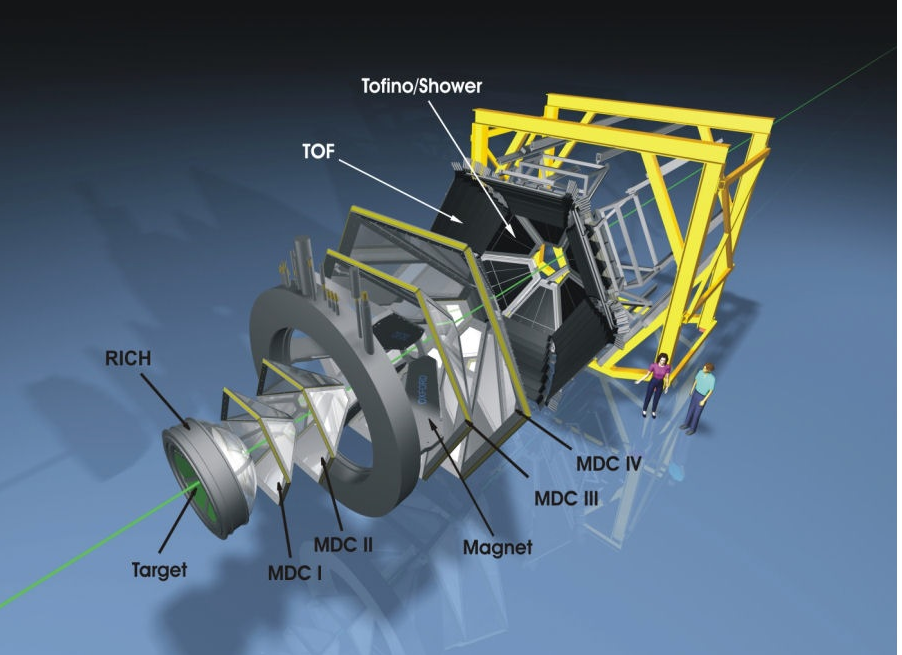
\includegraphics[width=120mm]{Hades}
	\caption{The schematic diagram showing HADES detector system.
	The subsystems - RICH, MDC, TOF/Tofino, Shower are composed of 6 constructionally 
	equivalent sectors. 
Such solution permits the full coverage (360$^{\circ}$) of the azimuthal angle.
The acceptance in the polar angle is assured for 18$^{\circ} < \theta < 85^{\circ}$.}
	\label{Hades}
\end{figure}

In the HADES experiment the stationary targets are used. 
This fact creates the need to extend the detection apparatus towards forward emission 
angles in the laboratory reference frame. 
HADES detection system has full symmetry along the azimuthal detection angle. 

The target system is embedded by the construction of the Ring Imaging Cherenkov detector (RICH) 
used for detection of leptons.
For registration of charged hadronic reaction products the set of Multiwire Drift Chambers (MDC) 
and the scintillating walls called TOF and Tofino are utilized. Electromagnetic calorimetry 
is performed by the electromagnetic shower detector installed at the end of detection system.
Each of the detection subsystem is composed of 6 equivalent sectors. 

%The following particles are of interest for studying the mechanism of p+Nb reactions at 3.5 GeV proton beam energy: $\pi^+$, $\pi^-$, p, d, and t. 

In the HADES experiment the registration and identification of $\pi^+$, $\pi^-$, $p$, $d$, and $t$ created in the target  
is performed by the set of Multiwire Drift Chambers (MDC) and the TOF/Tofino scintillating walls.
The momenta of particles are analyzed by magnetic field created by toroidal superconducting magnet.
The cross section of HADES apparatus used for measurement of $p+Nb$ reaction at 3.5 GeV 
is shown in fig. \ref{HadesV2}.

\begin{figure}
	% Requires \usepackage{graphicx}
	\centering\
	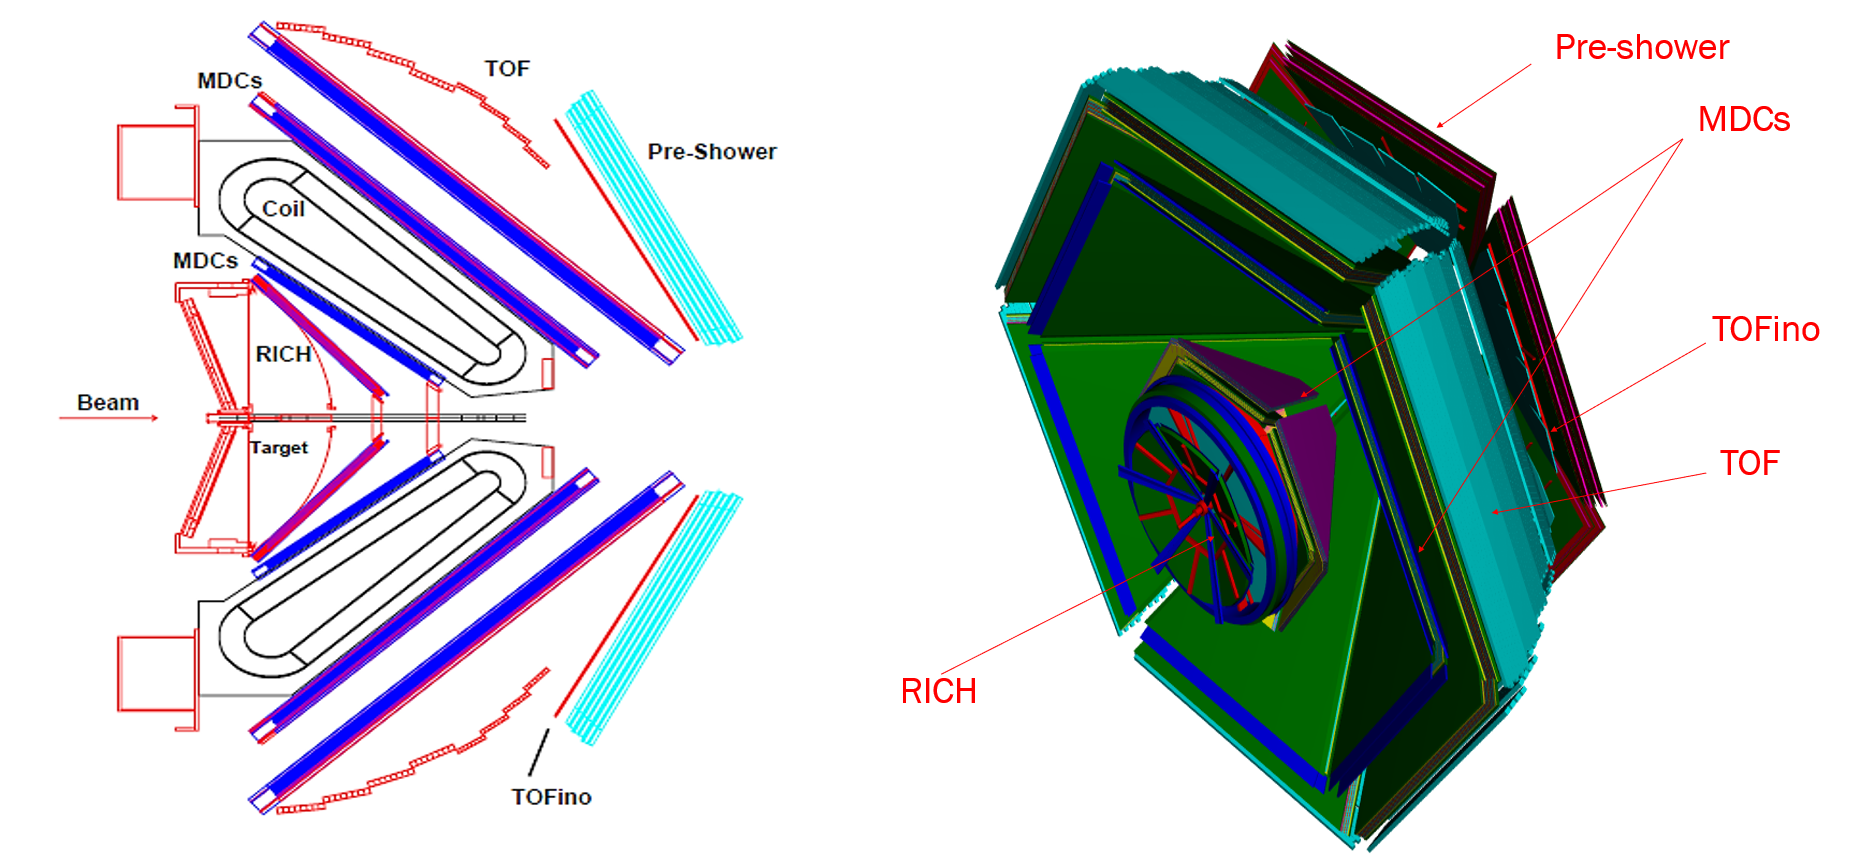
\includegraphics[width=120mm]{HadesV2}
	\caption{The cross section of the HADES apparatus used for  
measurement of $p+Nb$ reaction at 3.5 GeV. The most important 
detection subsystems for registration of $\pi^+$, $\pi^-$, $p$, $d$, and $t$, 
are the Multiwire Drift Chambers (MDC) and TOF/Tofino scintillating walls. 
MDC are the tracking detectors. They provide also the information about the specific 
energy losses of particles. Scintillators measure as well the energy loses 
but they work also as triggering detectors.
The momenta of particles are measured with the use of magnetic field 
of a superconducting magnet. The toroidal magnet is installed between the pairs of MDCs.}
\label{HadesV2}
\end{figure} 


\subsection{Target}

The solid target of $^{93}Nb$ has been used. 
The construction of the target is as follows. 
It consists if the segments installed coaxially along the beam axis.
The diameter of each segment was equal to 2.5 mm and its thickness was of 0.45 mm.
The distances between segments were equal to 4.5mm. Such construction of target was optimized in order to enhance the total luminosity 
for the dilepton studies. 
In case of spallation products which are of interest of this work important is only the 
central segment of the target \ref{Z-coordinate}. The pions and nuclear products created in the segments of target 
located more upward the beam than the last segment do not contribute to the registered spectra 
since they are dumped inside the target (????)
\begin{figure}[H]
    \centering
    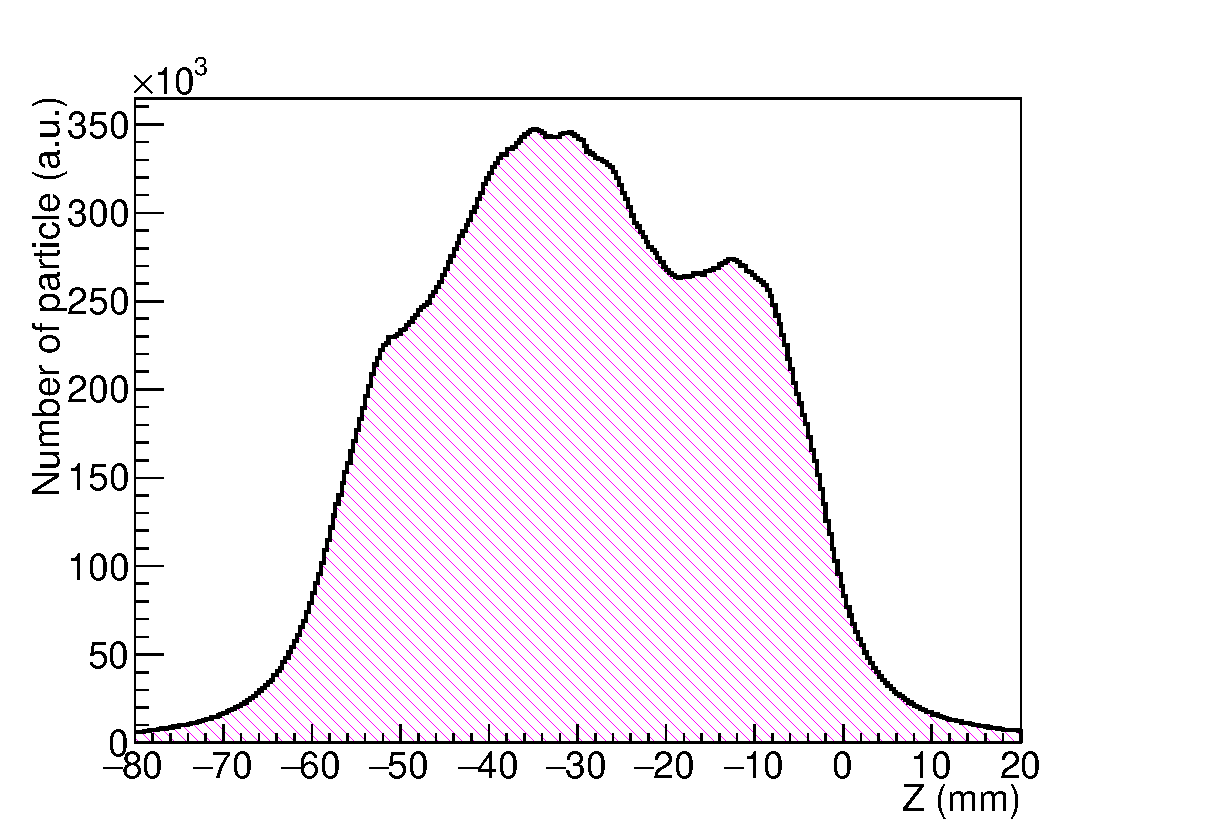
\includegraphics[width=0.6\textwidth]{Z-coordinate_target.eps}
    \caption{Caption}
    \label{Z-coordinate}
\end{figure}
.....

.....


\subsection{Mini Drift Chamber (MDC)}
The tracking system of HADES is constructed from 24-trapezoidal MDC modules. 
They are arranged symmetrically in $\phi$ angle around the beam axis. 
Each individual detection sector consists 4 modules -  two before 
the toroidal super conducting magnet and two after the magnet.
The sizes of the modules increase when proceeding to the forward direction. 

The individual drift chamber (one module) is constructed of six layers. 
The angular orientation of the sense (anode) wires of each layer is different. 
The sensing wires are soldered at +40$^\circ$,  -20$^\circ$, +0$^\circ$, -0$^\circ$, +20$^\circ$ and -40$^\circ$ 
with respect to direction perpendicular to the beam axis.It is shown in fig. \ref{mdc}.   

The sense wires are made of tungsten which is plated with gold. 
For plane I-III the thickness of anode wires is 20 $\mu$ m whereas for the last IV plane 30 $\mu$ m.
Constant mechanical wire tension of 40 cN and 50cN, respectively, is used. 

The cathode wire are made of 80-110 $\mu m$ annealed aluminum 
(bare - plane I-III or gold plated -plane IV). 
The exact diameter of cathode wires increase with the size of chamber.
The same concerns the mechanical tension of cathode wires which varies between 150 and 180 cN.

The entrance windows of  MDCs are made from 12$\mu m$ aluminized mylar foils.

Chambers was filled with helium-isobutane gas mixture in the proportion of 60:40. They work at atmospheric pressure.  

Position resolution of MCD system is $\le$ 100 $\mu$m in polar angle direction and $\le$ 200 $\mu$m 
in azimuthal angle direction. This permits the precise tracking and momentum reconstruction 
with the resolution of of $\delta{p}/p$ $=$ 4\%.

The effective thickness of the whole set of MDC modules is of 0.5\% of the radiation length. 
Despite of such small thickness the MDC are able to provide precise information 
about particle's energy losses. The resolution of the measured energy loss per path length, 
d$E$/d$x$, is of 7\%. The value of energy loss is measured by means of Time over Threshold 
of the detector signal \cite{Kipnis}. 
The distributions of d$E$/d$x$ vs momentum are crucial for particle identification by means 
of their specific energy losses.

\begin{figure}
	% Requires \usepackage{graphicx}
	\centering
	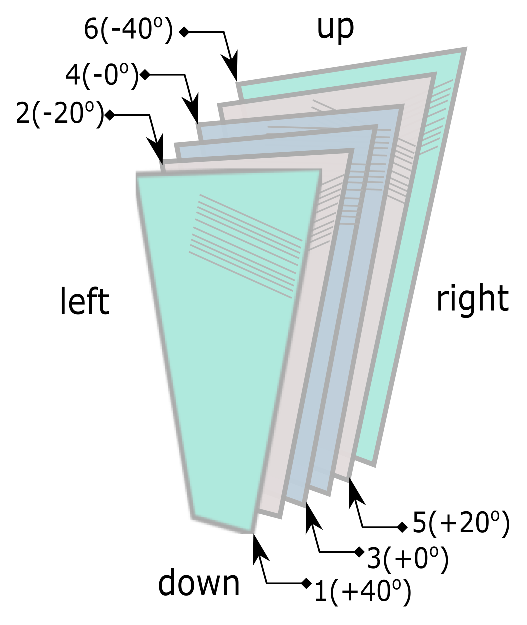
\includegraphics[width=0.45\textwidth]{mdc.eps}
	\caption{Schematic view of the sequence of six layers of each module of drift chamber 
	and the angular orientation of the sensing wires of each layer.}
	\label{mdc}
\end{figure}



\subsection{Superconducting Magnets}

The HADES detector comprises the 6 coils of superconducting magnets surrounding the beam axis. 
Each coil is kept in individual vacuum chamber. 
%The vacuum chambers were also connected to support a ring in which target is placed. 
In each coil maximum field 3.6 T can be generated. 
The magnetic filed of each sector was mapped with the use of a Hall probe 
and a devoted optical positioning system. 
%This mapped field also implemented into HYDRA (detector simulation tool) which is later used in efficiency calculations.    

\subsection{TOF/TOFino}

The TOF and Tofino detectors despite of their names were not used for Time-of-Flight measurement.
In the measurement of the $p+Nb$ reaction the START detector installed in vicinity of the target could not be operated.
For this reason the TOF and Tofino scintillating walls were utilized only as a trigger detectors. 
But they are able to provide as well the precise information about energy loss of registered particles. 
This advantage has been utilized in this work.

The TOF scintilating wall covers the $\theta$ angular range from 44$^{\circ}$ to 85$^{\circ}$. 
Each sectors comprises 8 modules of TOF detector. Each such detector consists of 8 strips of plastic scintillator. 
The thicknesses of the strip depends on their angular position and varies between 20 and 30 mm.
The time resolution of TOF scintillators is equal to 150 ps. Their position resolution is equal to 3 cm.
This results in the excellent d$E$/d$x$ resolution of the TOF detector of 4\%.  

The Tofino scintillating plastic paddles covers the gap between 18$^{\circ}$ and 45$^{\circ}$ of $\theta$ angle.
There are only 4 individual detector per one sector. 
Signals of these detectors are readout only at one side of the paddle. This results 
in the worse timing and energy resolution of Tofino walls than in cose of TOF. 
They are equal to 420 ps and 8\% respectively.
The double hit resolution of Tofino is worse than this of TOF as well.


\subsection{Triggering}

Data Acquisition System (DAQ) in HADES experiment record the data in the event-by-event regime. 
During the collection of the data from $p+Nb$ reaction at 3.5 GeV the two independent sequences of signals triggered the (DAQ).

\begin{itemize}
\item The first trigger aimed in selection of hadronic reaction products. It required a signals of at least 3 charged particles were registered 
in TOF and/or TOFino detectors.  
\item The second trigger were constructed for identification of dileptons. The triggering condition were fulfilled if two electron signatures have been
identified in the RICH detector.
\end{itemize}

Only the first trigger were sensitive for signals from charged pions and $H$ isotopes. 
Thus, only this trigger condition is important for the goal of the present examination.

\subsection{Software tools for tracking and simulation of detector response}

The tracking algorithms of HADES take into account the mapped magnetic field of toroidal magnet.

.....


\begin{figure}
	% Requires \usepackage{graphicx}
	\centering
	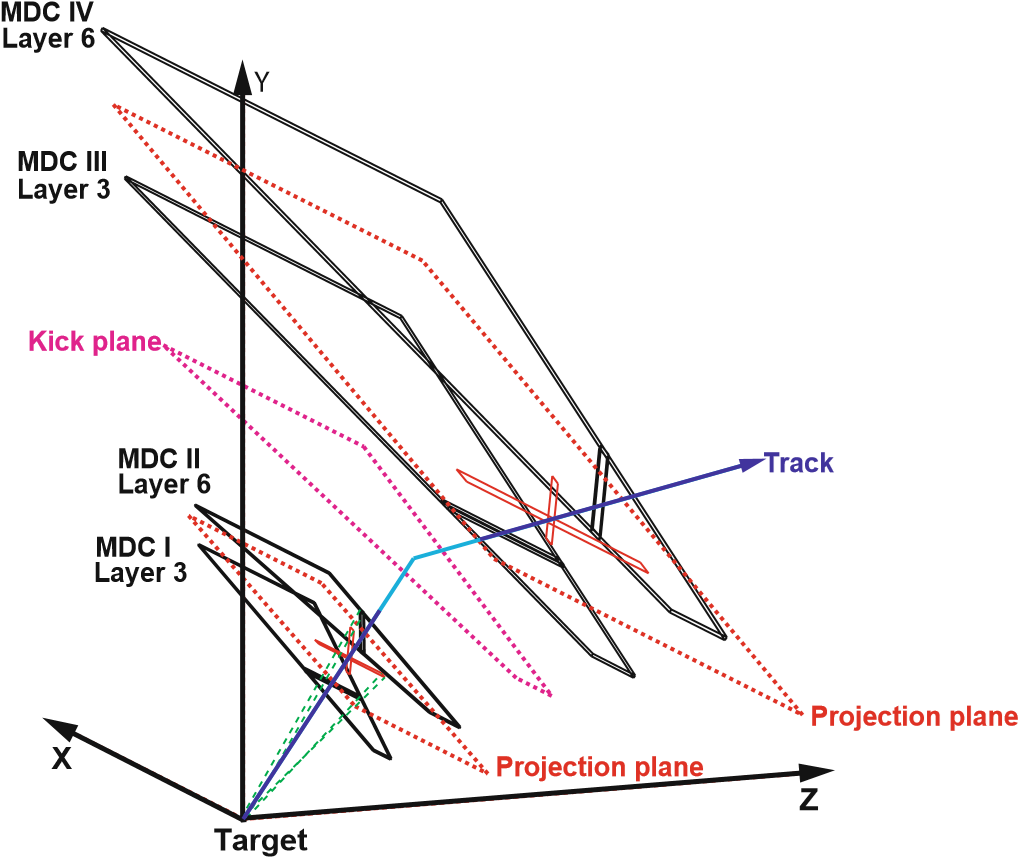
\includegraphics[width=0.65\textwidth]{tracking}
	\caption{Schematic view of track reconstruction using MDC detectors. Only one layer of the MDC detector is shown to simplifying the diagram.  }
	\label{tracking}
\end{figure}


The acceptance of the total and each of the subdetection system is simulated 
by the hGeant software module.

.....

The simulation of response of of the detection system including the trigger conditions, the tracking algorithms, energy losses, efficiences 
and demanded calibrations is provided by the Hydra software.   


.....


 




















The Ring Imaging Cherenkov (RICH) detectors and the Pre-shower detectors shown in fig. ref{HadesV2} have not been used for the current studies, 
thus their description is avoided in this thesis. The reader interested in these subsystems is asked to referee to \cite{agakichiev2009HADES}.


 \ \\
 
 CORRECTED UNTIL HERE
 
 
 \ \\


% The experiment was performed at GSI Darmstadt. 
% The identification of particles was done using various detectors like \textbf{M}ini \textbf{W}ire \textbf{D}rift Chamber (MDC) and \textbf{T}ime \textbf{O}f \textbf{F}light detectors (TOF). The main issue was to proper estimation of background in case of d, t and the absolute normalization, taking into account the detection acceptance, efficiency, and trigger conditions.
% \section{p+ Nb @ 3.5 GeV measured in HADES@GSI}


% The main goal of this investigation was to identify and select light charged products $\pi^+$, $\pi^-$, p, d, and t from p + Nb experiment by taking the advantage of the high resolving power of particle identification in HADES. For checking the quality of data the results obtained at HADES were compared with cross sections obtained in similar conditions by HARP experiment [ref]. 
% 
% The obtained in experiment double differential cross sections were used for validation of several theoretical models i.e. INCL++, UrQMD and GiBUU.

% \subsection{Solution of various challenges in Raw Data Analysis}
% There was no start detector in this experiment, thus time was reconstructed using fast reference particle (in this case. Therefore, the time-of-flight information (beta) can't be used for identification of single spectra. Particle the identification (PID) is done based on dE/dx information only (from MDC and TOF, TOFINO). Trigger: 3 or more charged particles not optimal for single spectra. Simulations are used to make trigger corrections   


%\section{Description of experiment}
% The goal of the experiment was to measure coincidences of di-electron pairs with the light charged particles emerging from proton-nucleus collisions.  In the on-line storage of events  two levels  trigger was used. The first-level trigger selected all events in which at least 3 charged particles were detected in TOF and/or TOFino detectors.  The second- level trigger accepted only the events with electron signatures from RICH detector.   Since the data were stored in the event-by-event format, it is also possible to select them for coincidences appearing between the detection of light ions  among themselves as well as with pions.  Due to this, it is possible to achieve the information necessary for studying the spallation reactions induced by protons. In the online storage of events, there is used two-level trigger: The first level trigger is a multiplicity trigger of at least 3 charged particles detected in TOF and/or TOFino. The second level trigger is obtaining electron signatures (from RICH). 

% \subsection{Ring Imaging Cherenkov(RICH)}
% This is inner most part of HADES detector system. It is hadron blind detector designed to detect e$^\pm$  with momentum in range  0.1-1.5GeV/c. The schematic view of RICH detector system is shown in figure \ref{RICH}. This detector is placed in very limited space of target and tracking system. The detector was filled with radiator gas perfluorobutan (C$_2$F$_10$) which offer high transmission till low wavelength $\lambda= 145nm$. It also has Cherenkov threshold to suppress radiation from muons and hadrons in given momentum range. The Cherenkov light is emitted from straight particle trajectory with path length ranging from 36 cm at $\theta=20^\circ$ to 65 cm at $\theta=80^\circ$. Which is reflected by low mass spherical mirror having curvature radius R= 872mm. Photon reflected from spherical mirror are transmitted through the  CF$_2$ widow into gaseous photon detector. The photon detector has CsI as cathodes with six Multi-Wire Proportional Chamberers(MWPC) filled with CH$_4$. Each MWPC has individual pad readout.
% \begin{figure}
% 	% Requires \usepackage{graphicx}
% 	\centering\
% 	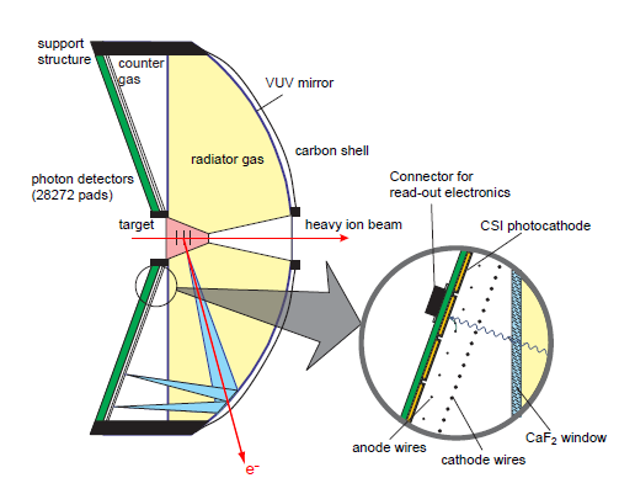
\includegraphics[scale=0.65]{RICH}
% 	\caption{In this figure various parts of RICH detector is shown }
% 	\label{RICH}
% \end{figure}



\section{Methodology of data analysis}
The identification of H isotopes and charged pions among the data registered in HADES during $p+Nb$ run at 3.5 $GeV$ encountered two significant difficulties which are not present in the selection of the "conventional" leptonic or hadronic products of the interest of the HADES collaboration.

\begin{itemize}
	\item The trigger system permitted to register the events where at least 3 charged particles have been detected in the TOF/TOFino walls. For the current analysis this fact implicated the following difficulties:
	(i) the purely single distribution spectra were not registered. Instead, each detected event comprised at least three charged particles including secondary and primary various particles.
	(ii) the trigger system was insensitive to the origin of the triggering particles. The trigger conditions could be fulfilled by detection of both the reaction products originating from the target as well as by the secondary particles created in the elements of the setup.
	\item The lack of the START detector for the Time of Flight (TOF) measurement influences a lot the identification strength of the HADES detection system for the reaction products which are subject of the current investigation. In view of the missing start detector, the (TOF) of the selected particle could be reconstructed by the comparison to the (TOF) of the fastest identified particle of the event. But as long as the single distribution of reaction products are of interest the coincidences with other particles have to be disregarded. For this reason the identification 
	based on the mass-momentum dependence could not be utilized in the current analysis. 
	This method was used only for the identification of the first level cuts and for the preselection of the data.
	The lack of knowledge of the $\beta$ value of selected particles significantly reduced the energy ranges for $\pi{^+}$, $d$ and $t$ where these particles could be identified. 
\end{itemize}
\subsection{\label{PID} Particle identification and background subtraction}
As mentioned above rely on the beta values for single spectra. Thus beta information is only used to define the $dE/dx$ identification cuts. The following methods had been applied for the identification of particles:
\begin{itemize}
	\item The mass distribution is calculated from the beta value (shown in figure \ref{MassCuts}). Which is  reconstructed TOF detector and from the fast particle(i.e $\pi^{-}$) have been used only at the beginning of data analysis to predefined the identification cuts for dE/dx vs momentum for MDC and TOF/TOFINO detectors show in figure \ref{MassCuts}.
	\begin{figure}
		% Requires \usepackage{graphicx}
		\centering
		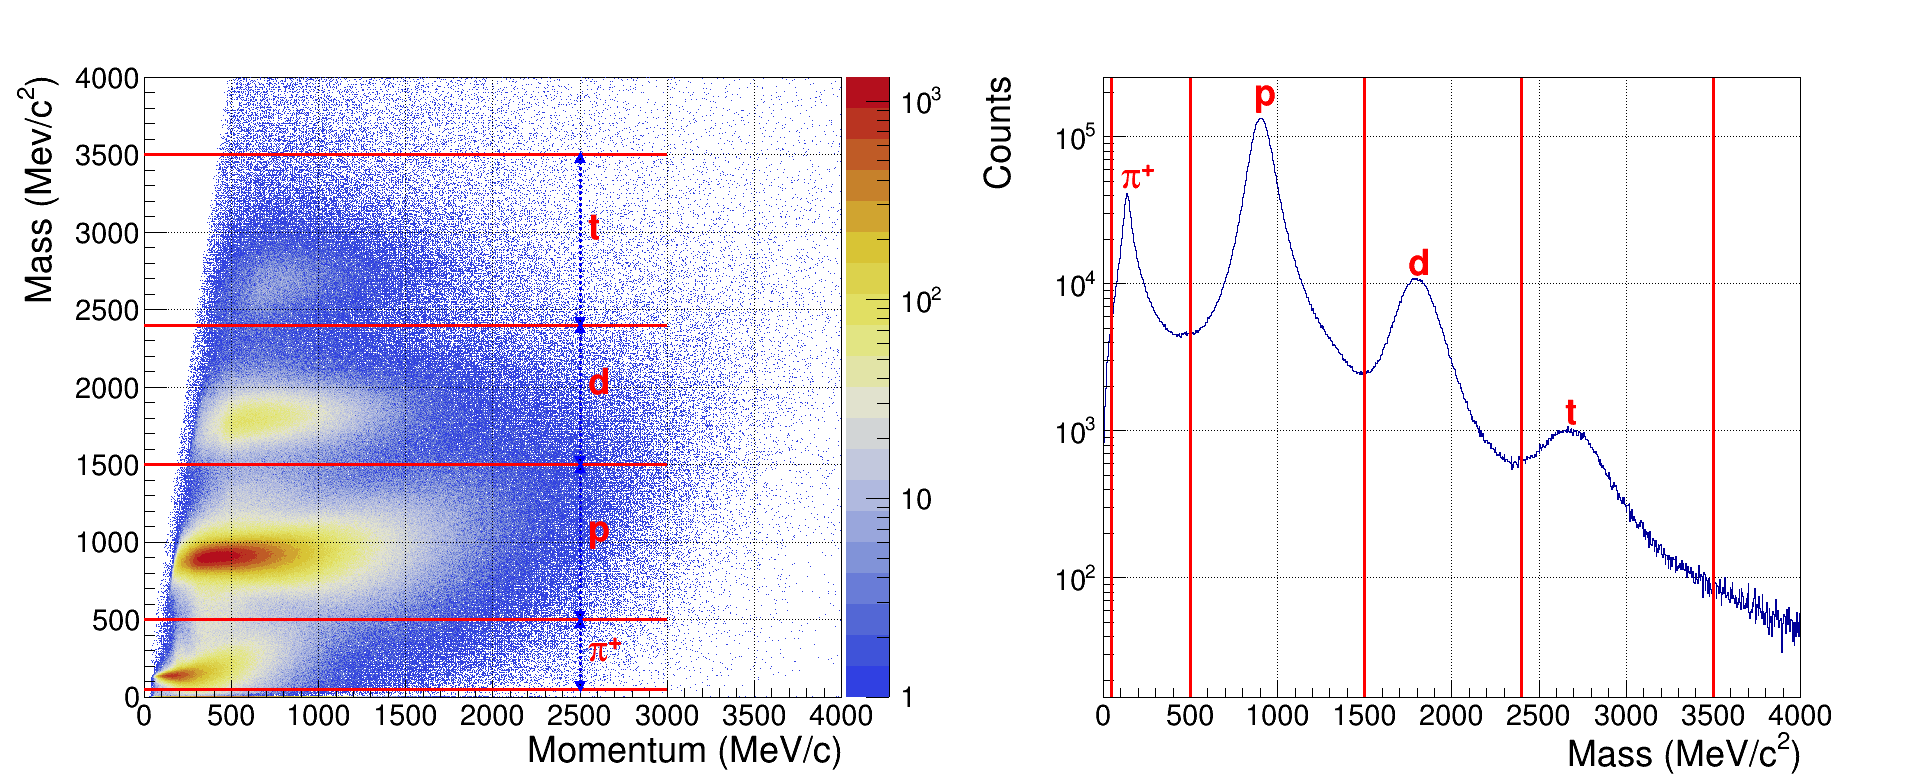
\includegraphics[width=0.95\textwidth]{MassCut.png}
		\caption{The mass distribution calculated from the beta value is shown in lef}
		\label{MassCuts}
	\end{figure}
	\item After applying the mass cuts(shown in figure \ref{MassCuts}) for p,d,t,$\pi^+$ the dE/dx vs momentum spectrum is plotted. Then the projection of y-axis for 25MeV energy bin has been taken(Example of proton for momentum bin 725-750 MeV projection is shown in figure \ref{Projec})
	\begin{figure}
		% Requires \usepackage{graphicx}
		\centering
		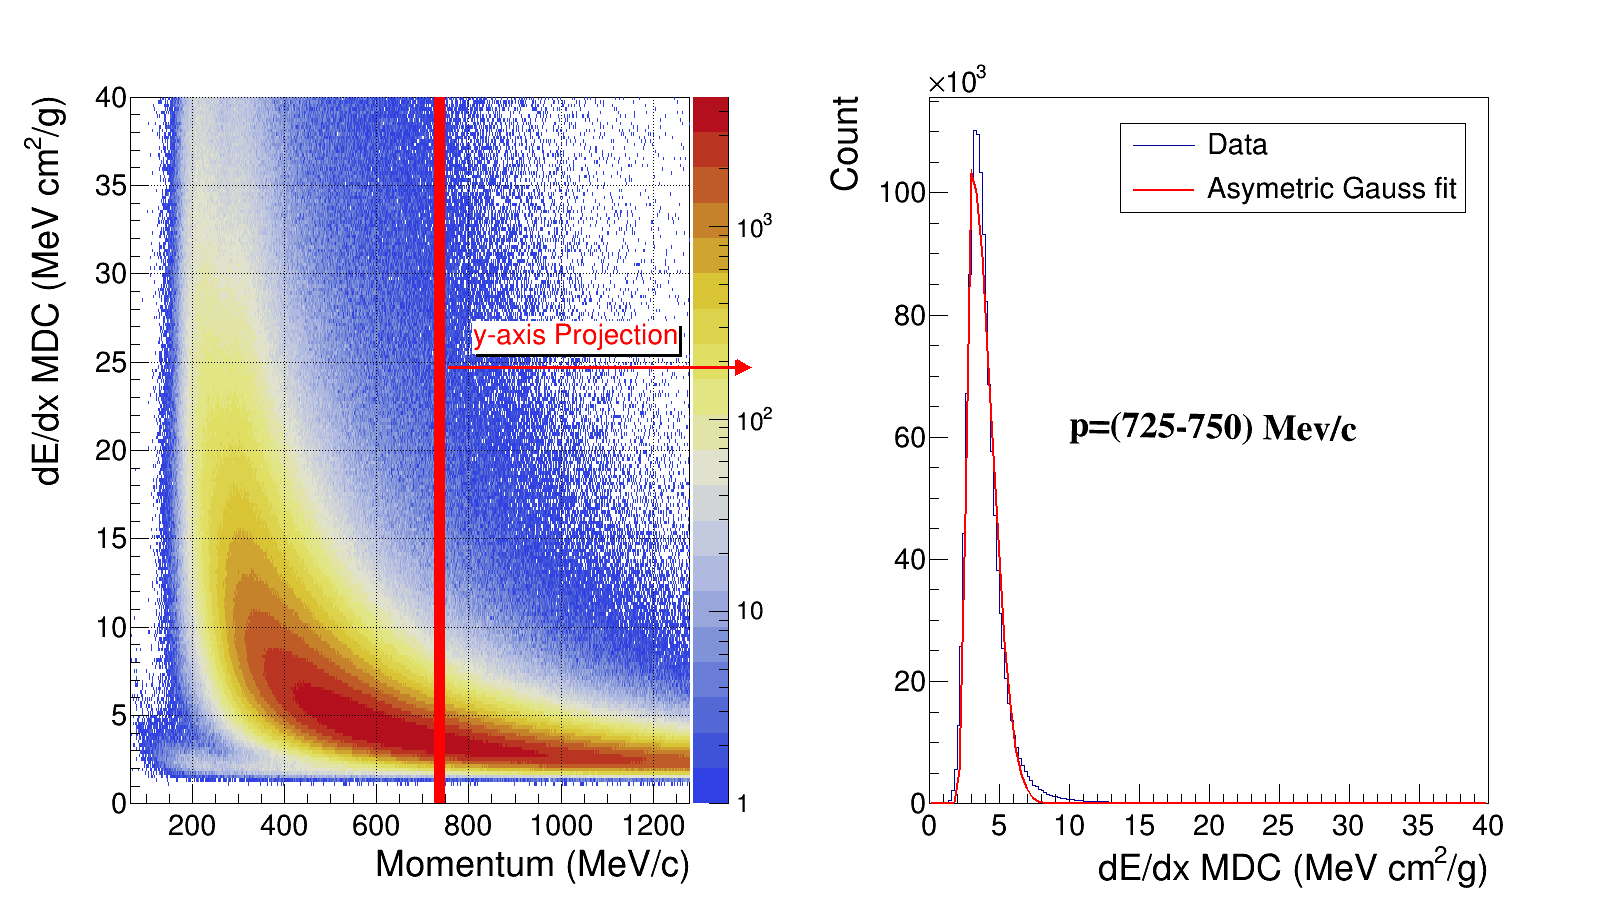
\includegraphics[width=0.95\textwidth]{projection.png}
		\caption{In this figure various parts of RICH detector is shown }
		\label{Projec}
	\end{figure}
   \item Then asymmetric Gaussian (ref \ref{aGauss}) function is fitted for every 25 Mev energy bin. For example in figure \ref{Projec} proton MDC dE/dx spectra y-axis projection for momentum bin (725-750)MeV is fitted with asymmetric Gaussian function.  
   \begin{equation}
   	f_g(x)=\begin{cases}
   		\frac{1}{\sigma_l\sqrt{2\pi}}e^{-\frac{1}{2}\left(\frac{x-\mu}{\sigma_l}\right)^2}&\mu\le0\\
   		\frac{1}{\sigma_r\sqrt{2\pi}}e^{-\frac{1}{2}\left(\frac{x-\mu}{\sigma_r}\right)^2}&\mu>0
   	\end{cases}
   \label{aGauss}
   \end{equation}
   \item The determined mean $\mu$ and two sigmas (left/right) values are used to determine the various width of MDC cuts shown in figure \ref{MDCcut}. Here the only example of three widths are shown ($\mu \pm \sigma_i \times m$) where i is r and l for left sigma and right sigma respectively and m is the multiplier for five different widths which is taken as 0.6, 0.8, 1.0, 1.2, 1.5. In figure cuts for three m values are shown.
   \begin{figure}
   	% Requires \usepackage{graphicx}
   	\centering
   	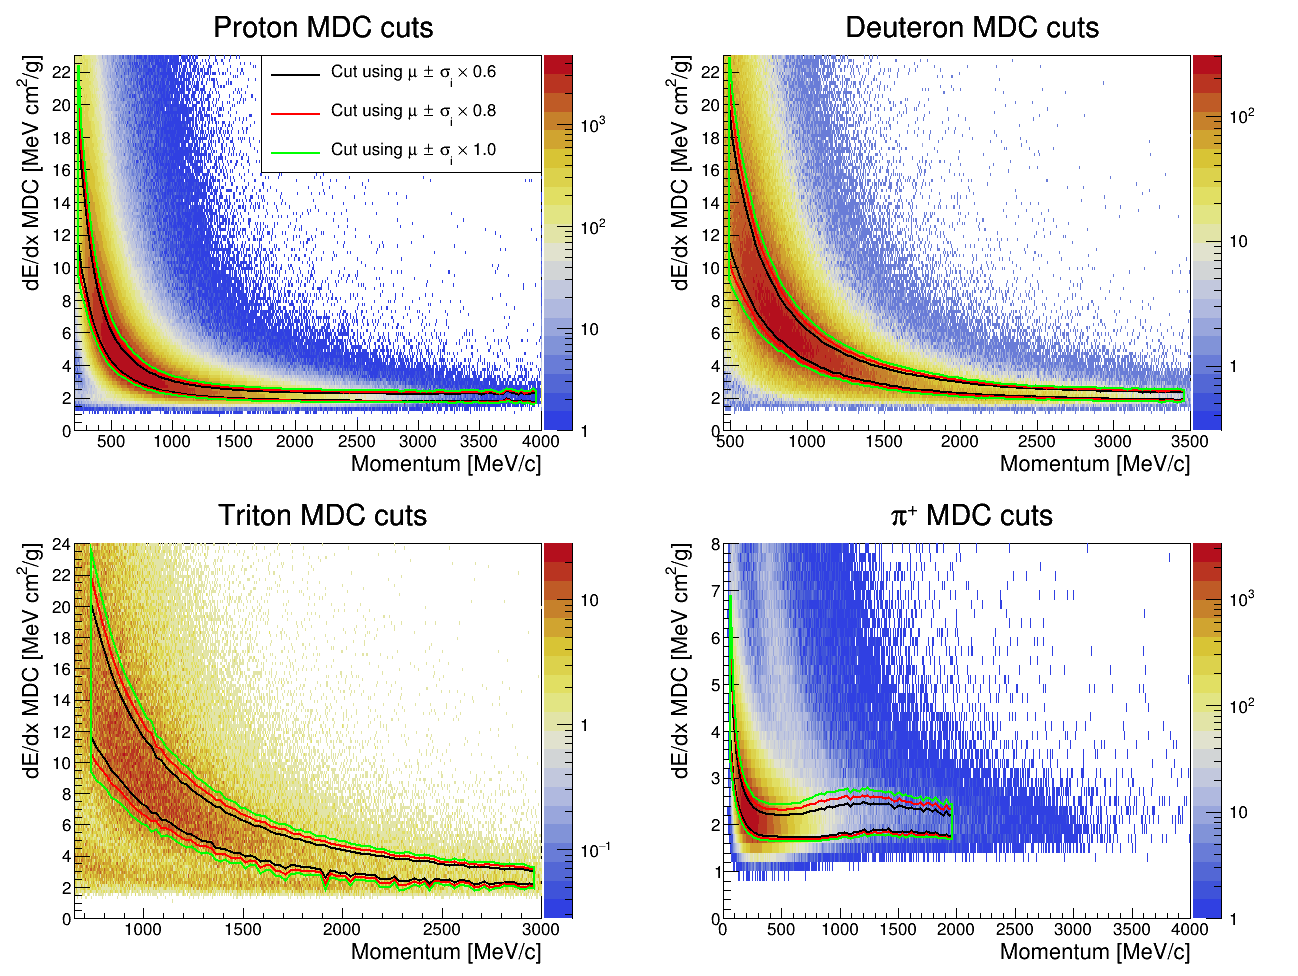
\includegraphics[width=0.95\textwidth]{MDC_CUTS.png}
   	\caption{The scatter plot of dE/dx (MDC) vs. momentum for protons. The cut obtained from 
   		the asymmetric Gaussian fits is shown. The theoretical calculation of energy loss according to Bethe-Bloch formula is shown as well with the red line.}
   	\label{MDCcut}
   \end{figure}
  \item After determining the MDC cuts both the cuts from MDC  dE/dx and mass cuts are used to plot dE/dx vs momentum distribution for TOFino($18^o-40^o$ angle) and TOF($45^o-85^o$ angle). Then again y-axis projections having a bin width of 25 MeV momentum are taken and fitted with asymmetric Gaussian function.
  \item Using the similar procedure as mentioned above various withs of dE/dx cuts for, m = 0.6, 0.8, 1.0, 1.2, 1.5, 1.8 are determined for TOF/TOFino defectors.
  \item In this way (after demanded smoothing) the 2D cuts ($dE/dx - momentum$ plain) for all positively charged reaction products of interest have been created and applied to the raw data to select the experimental distributions.
  \item The separation of negatively charged pions from other reaction products is provided by their opposite deflections in the magnetic field. Thus there was no need for the definition of the cuts for their identification. The contamination of the $\pi^{-}$ spectra with the $K^{-}$ is insignificant and disregarded here.
\end{itemize}

To determine the background of the particle following methods had applied:
\begin{itemize}
	\item Firstly MDC cuts are applied which is determined in the above text then again TOF/TOFino detector dE/dx vs momentum distribution for angles (20,25,30,...$85^o$)  is plotted. The corresponding width of cuts(for m = 0.6, 0.8, 1.0, 1.2, 1.5, 1.8) are applied to determining the background in each width of TOF/TOFino cuts.
	\item After plotting a distribution for a particular angle and with of cuts for TOF/TOFino detectors. The distributions of selected particles (within the cuts) after their projections to $dE/dx$ axis the fits of signal and background distributions have been performed for a given in range of ($\mu-\sigma_l*m , \mu+\sigma_r*m$) where m = 0.6, 0.8, 1.0, 1.2, 1.5, 1.8 and sigma values are taken from earlier fits. For example background calculation for p, d, t, and $\pi^+$ at angle $\theta=25$ and width $\mu \pm \sigma_{l/r}\times1.5$ is shown in figure \ref{backg}.
	\begin{figure}
		\centering
		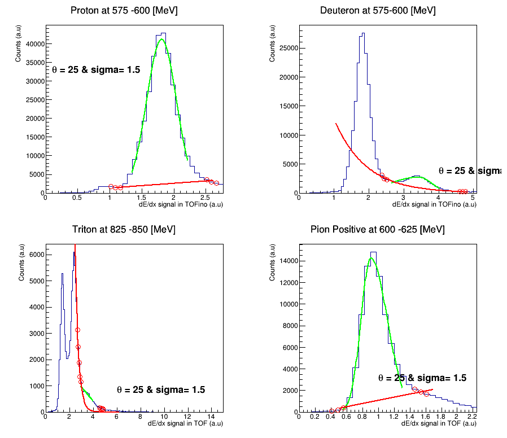
\includegraphics[width=0.95\textwidth]{PidBackground.png}
		\caption{Background}
		\label{backg}
	\end{figure}  
\end{itemize}



\subsection{\label{Eff_corr} Efficiency corrections}
In order to absolute normalization of the cross-section the overall efficiencies of different particles i.e p, d, t, $\pi^-$ and $\pi+$ was determined. In the case of the current study, it is a product of detection efficiencies of various components of the HADES system, the effectiveness of the data acquisition system, the trigger conditions and the distributions of secondary particles created in the HADES setup and contributing to the triggering of event. The total efficiency is depended on energy, theta and type of particle.





% \begin{figure}
% 	% Requires \usepackage{graphicx}
% 	\centering\
% 	\includegraphics[width=0.95\textwidth]{INCLEff}
% 	\caption{The scatter plot of dE/dx (MDC) vs. momentum for protons. The cut obtained from 
% 		the asymmetric Gaussian fits is shown. The theoretical calculation of energy loss according to Bethe-Bloch formula is shown as well with the red line.}
% 	\label{INCLEff}
% \end{figure}
% \begin{figure}
% 	% Requires \usepackage{graphicx}
% 	\centering\
% 	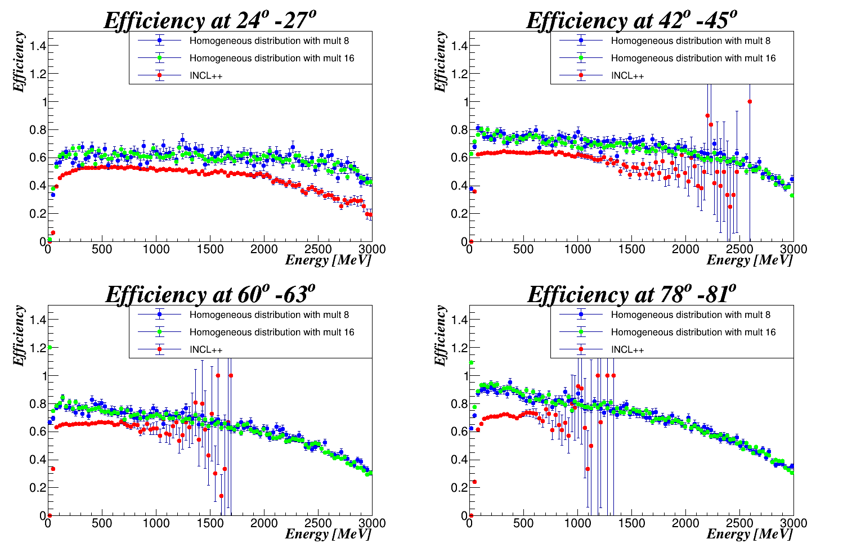
\includegraphics[scale=0.6]{Efficiency}
% 	\caption{The scatter plot of dE/dx (MDC) vs. momentum for protons. The cut obtained from 
% 		the asymmetric Gaussian fits is shown. The theoretical calculation of energy loss according to Bethe-Bloch formula is shown as well with the red line.}
% 	\label{Eff}
% \end{figure}
% \begin{figure}
% 	% Requires \usepackage{graphicx}
% 	\centering\
% 	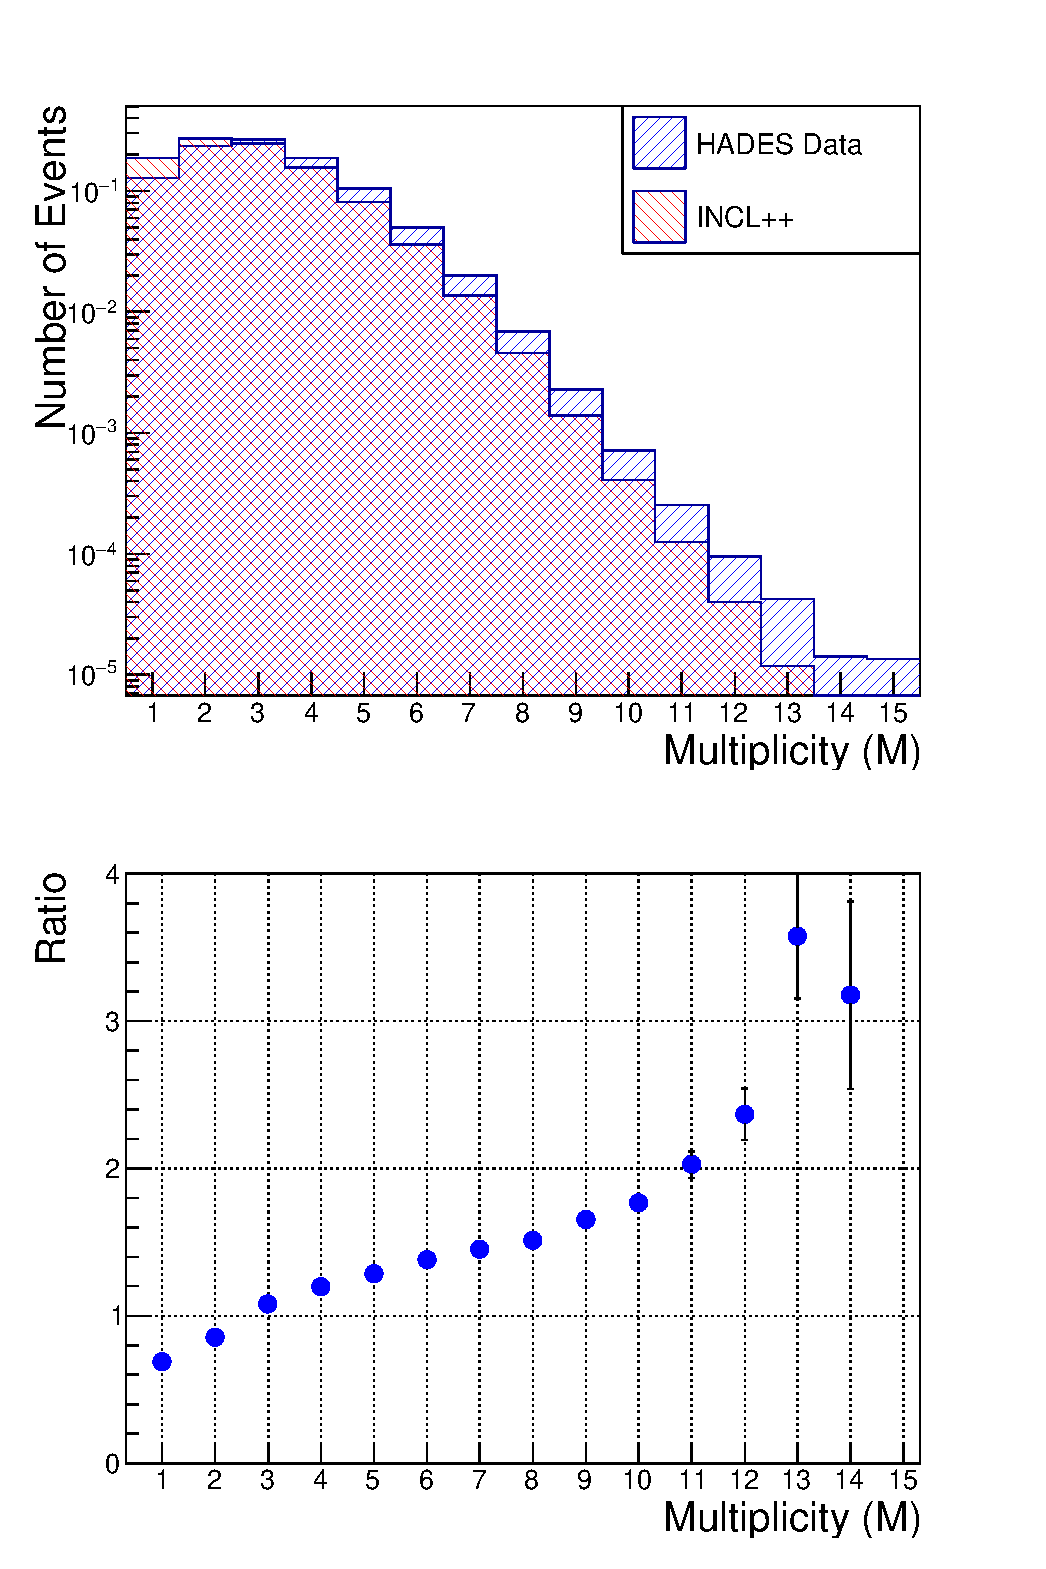
\includegraphics[width=0.95\textwidth]{MultINCL}
% 	\caption{In this figure various parts of RICH detector is shown }
% 	\label{MultINCL}
% \end{figure}
% \begin{figure}
% 	% Requires \usepackage{graphicx}
% 	\centering\
% 	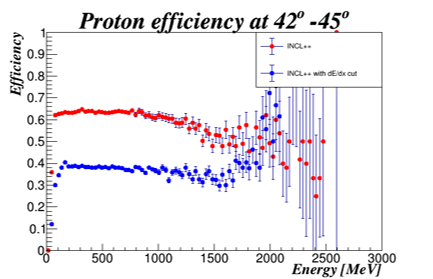
\includegraphics[width=0.95\textwidth]{Efficiency2}
% 	\caption{The scatter plot of dE/dx (MDC) vs. momentum for protons. The cut obtained from 
% 		the asymmetric Gaussian fits is shown. The theoretical calculation of energy loss according to Bethe-Bloch formula is shown as well with the red line.}
% 	\label{Eff2}
% \end{figure}
% \begin{figure}
% 	% Requires \usepackage{graphicx}
% 	\centering\
% 	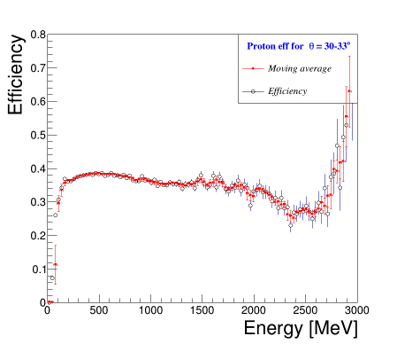
\includegraphics[width=0.95\textwidth]{runningAverage}
% 	\caption{The scatter plot of dE/dx (MDC) vs. momentum for protons. The cut obtained from 
% 		the asymmetric Gaussian fits is shown. The theoretical calculation of energy loss according to Bethe-Bloch formula is shown as well with the red line.}
% 	\label{RA}
% \end{figure}
\textbf{Secondary particles}:
The problem of secondary particles is resolved by tracking system(discussed in section [ref]). Since tracking system track back the particle from first MDC to TOF detectors. Secondary particles generated in random direction and randomly from any detection system can not form track through all four MDC modules and TOF doctors. This implies that these are particles are already removed in track reconstruction process
\begin{figure}
    \centering
\begin{tikzpicture}[node distance=1.2cm]
\node[draw,
    rounded rectangle,
    minimum width=2.5cm,minimum height=1cm , fill=red!30] (A){INCL++};
\node[draw,
    rectangle,
    fill=orange!30,
    minimum width=2.5cm,minimum height=1cm,below= of A] (B){HGeant};

\node[draw,
    rectangle,
    fill=orange!30,
    minimum width=2.5cm,minimum height=1cm,below= of B] (F){Hydra};

\node[draw,
    rectangle,
    fill=blue!30,
    align=center,
    text width=2.5cm,minimum height=1cm,below= of F] (E){$dE/dx$ vs $\theta$ histogram};

% \node[draw,
%     trapezium, 
%      fill=blue!30,
%     trapezium left angle = 65,
%     trapezium right angle = 115,
%     trapezium stretches,
%     minimum width=2.5cm,minimum height=1cm,below= of F] (E){$dE/dx$ vs $\theta$ histogram};

\node[draw,
    rectangle,
    fill=orange!30,
    align=center,
    text width=2.5cm,minimum height=1cm,below= of E] (D){Division};

\node[draw,
    rectangle,
    fill=blue!30,
    align=center,
    text width=2.5cm,minimum height=1cm,left= of D] (C){$dE/dx$ vs $\theta$ histogram};
% \node[draw,
%     trapezium,
%     fill=blue!30,
%     trapezium left angle = 65,
%     trapezium right angle = 115,
%     trapezium stretches,
%     text width=2.5cm,minimum height=1cm,left= of D] (C){$dE/dx$ vs $\theta$ histogram};
\node[draw,
    rounded rectangle, 
    minimum width=2.5cm,minimum height=1cm ,below= of D, fill=red!30] (G){Efficiency};


\draw[-latex] (A) edge
    node[pos=0.4,fill=white,inner sep=0]{Events} (B);
\draw[-latex] (A) -| (C) node[pos=0.4,fill=white,inner sep=0]{Events} (B) edge   node[pos=0.4,fill=white,inner sep=0]{Events}  (F);
\draw[-latex] (F) edge
    node[pos=0.4,fill=white,inner sep=0]{Events} (E) (C) edge (D) (E) edge (D) (D) edge (G);
  \draw [o->,blue] (C.east) -- (D);
  \draw [o->,blue] (E.south) -- (D);
\end{tikzpicture}
    \caption{Caption}
    \label{fig:my_label}
\end{figure}


\textbf{Trigger bias}:
\begin{enumerate}[label=\roman*)]
    \item To estimate the trigger bias various simulation were performed  using Hgeant with Isotropic emission  of proton  with different multiplicity(8,16) in single even.
    \item There are two tree of events, the generated events and the events which are detected in the detectors.
    \item These detected event then passes through the HYDRA framework which simulate  the trigger system , electronic behaviours and tracking effects.
    \item Then 2D histograms of energy vs theta are produced for generated events and final events after passing through the Hgeant and HYDRA.
    \item Efficiency of proton for Isotropic emission with multiplicity(8,16) is calculated by dividing 2D histogram of final events by generated events shown in figure \ref{IsoEff}.
    \begin{figure}
    \centering
	\begin{subfigure}[b]{0.45\textwidth}
		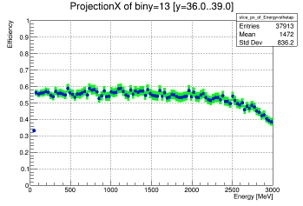
\includegraphics[width=\textwidth]{EffIsot8.png}
		\caption{\label{IsoEff8} Mutiplicity 8.}
	\end{subfigure}
	\begin{subfigure}[b]{0.45\textwidth}
		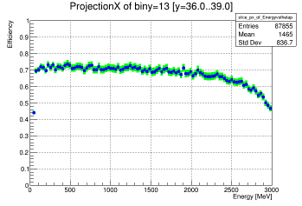
\includegraphics[width=\textwidth] {EffIsot16.png}
		\caption{\label{IsoEff16} Mutiplicity 16.}
	\end{subfigure}
	\caption{\label{IsoEff} Efficiency of proton for Isotropic emission with multiplicity(8,16) for $\theta =36^\circ-39^\circ$.}
\end{figure}
    \item The figure \ref{IsoEff} indicates that the efficiency is dependent on multiplicity of the particles in a events. This results suggest that we need a realistic models which can reproduce the multiplicity of particles which is same as it was in experiments.
    \item The results also suggest that dependence is not so strong from multiplicity 8  to 16. The change in efficiency is approximately 14\%.
    \item In order to produced realistic events as it was in experiments we choose INCL++ model. Then events are simulated for p + Nb @3.5 then these events are passed through HGeant and Hydra which simulate the detector behavior.
    \item Then comparison of multiplicity for INCL++ (passed through HGeant + HYDRA which is now equivalent to data) and Data are done and results are shown in figure \ref{MultINCL}.
    \item Since the efficiency with trigger condition not strongly depending on the multiplicity of charge particles. This implies that if we able to simulate reasonable multiplicity of charge particles we will able to simulate the trigger bias with HYDRA (using trigger condition on) framework.
    \item Using above arguments we can conclude that the trigger bias problem is resolved using the INCL++ simulation  as event generator and turning on trigger condition in HYDRA.
    \begin{figure}
	% Requires \usepackage{graphicx}
	\centering\
	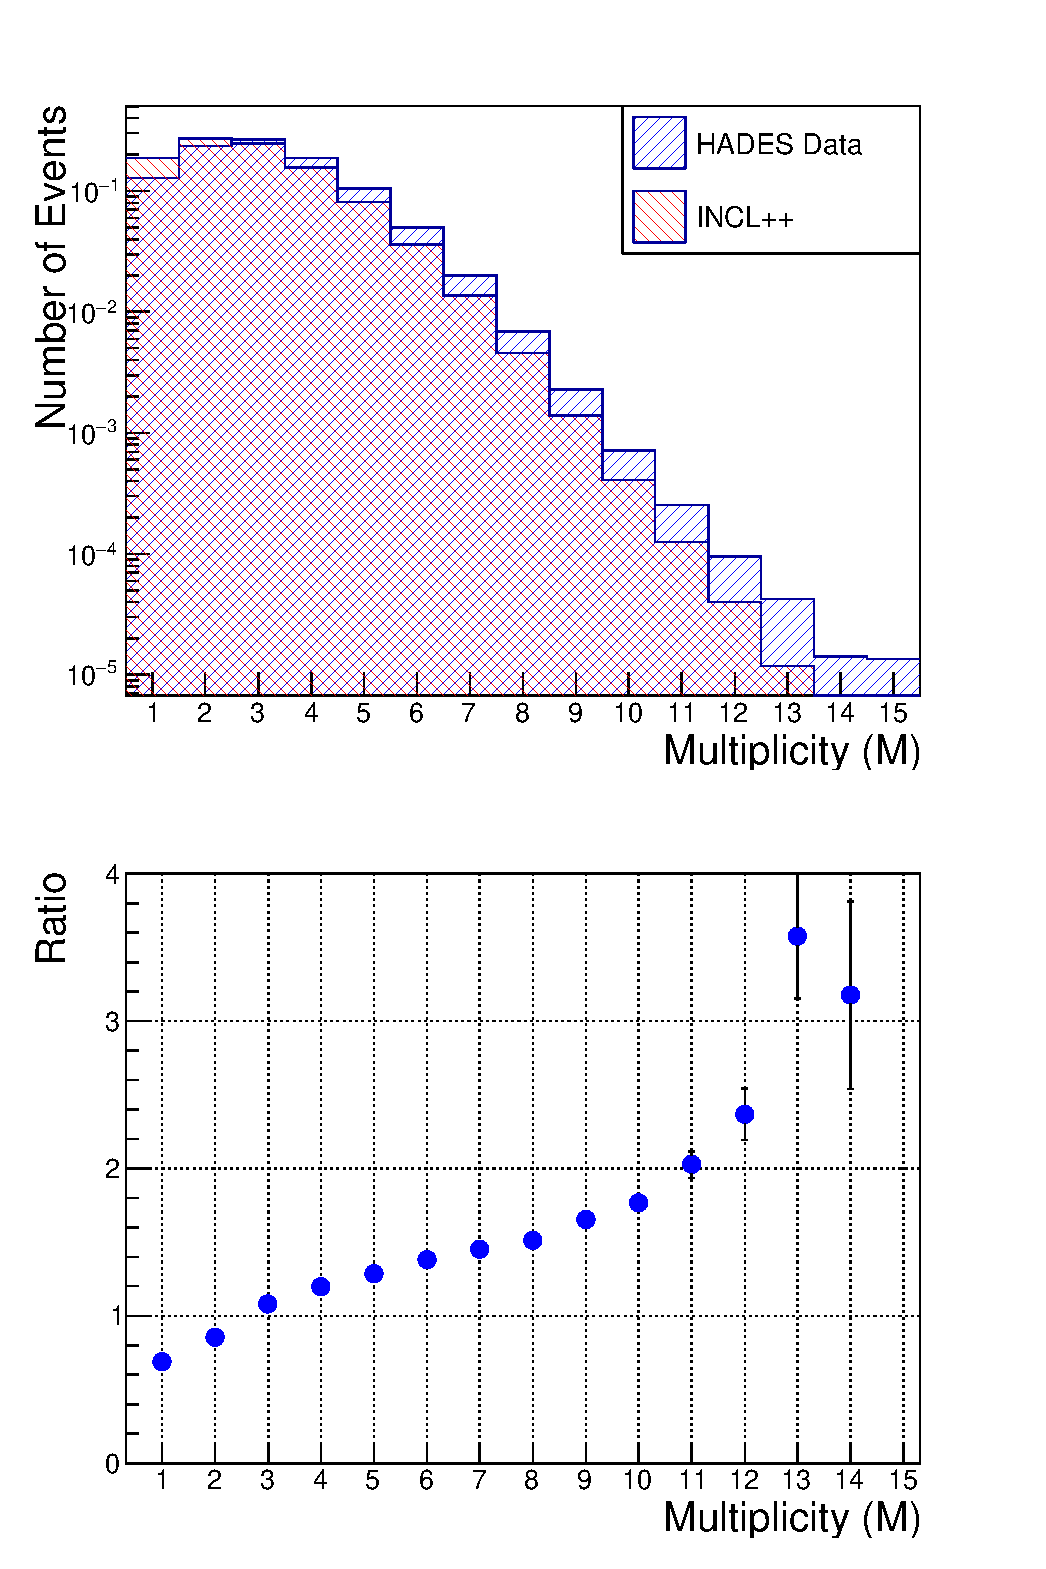
\includegraphics[width=0.6\textwidth]{MultINCL}
	\caption{In this figure multiplicity comparison between INCL++ and Hades data are shown }
	\label{MultINCL}
    \end{figure}
    \item From figure \ref{MultINCL} we can se INCL++ was able to reproduce the multiplicity of INCL++ shows reasonable agreement with the data. Which implies that reasonable  
\end{enumerate}
\subsection{\label{Uncertainties} Uncertainties}

The statistics of collected data is very high. For each energy bin of the presented data the statistical error 
is negligible and disregarded at the attached plots.

The components of systematic uncertainties come from: 
\begin{itemize}
	\item identification (definition of cuts, fit quality of the signal and background distributions, 
	uncertainty of background dispersion); 
	\item efficiency correction (applied event generator, limited statistics of simulations, bin-to-bin 
	dispersion of correction factors);
	\item differences of the response of individual sectors of HADES detection system;
	\item error of normalization factor used in HADES.  
\end{itemize}

Only the lasts component of the systematic error is constant and equal to 15\%. It was established in the former analysis 
of HADES pion spectra from $p+Nb$ collected at 3.5 GeV \cite{AgakishievPionP} and their comparison 
to the similar results of HARP-CDP collaboration \cite{Tlusty}. Other components are energy 
and emission angle dependent and will be shortly discussed below.  

\subsubsection{\label{pid/back} PID/background}

Due to lack of the clean mass identification based on the TOF information,  
the deconvolution of the signal and background events was based only on the specific energy loss method.
The resolving power of this approach is limited and varies with the energy of searched for particle.
In order to study the level of signal/background misidentification the whole procedure used for PID (as described 
in subsection \ref{PID}) have been performed for various widths of identification cuts. The applied cuts widths were of factor: 
0.6, 0.8, 1.0, 1.2, 1.5, 1.8 of the standard deviation $\sigma$ of the fitted asymmetrical Gaussian function (cf. fig \ref{PID_cut_1}). 
For each of the applied cut widths the net quantity of the signal events was calculated by subtraction of the background 
contribution from the signal one. 
The standard deviation of the average of all obtained results (for the given particle, emission angle and the energy bin) has been 
assigned as the systematic uncertainty of PID. For proton this component of error does not exceed 5\% for almost all energy range.  
%(???). 
The largest values of ...\% 
appear for the highest energies of (still resolved) tritons.

\subsubsection{\label{eff} Efficiency}

The efficiency correction method described in subsection \ref{Eff_corr} suffers from limitation 
of the used event generator, the limited precision of determination of particles momenta 
and limited statistics of simulations (especially for the highest energy regions). For the current issue 
it is important that the physics applied to create the generated events approximates 
the reality with sufficient precision. It was proved for INCL++ model. Since the method consists 
in dividing of two simulated distributions the effects of minor defficiencies of the model cancel out. 

It is known from the long term operation of HADES and from the other performed analyses 
that the overall efficiency of HADES 
varies smoothly with the energy of detected particle and with the emission angle. 
Thus, in the current studies only the energy regions where the efficiency changes 
monotonically were selected for the further analysis. 
The small fluctuations observed within the selected energy limits 
of the correction factors have been smoothed by applying of the running average 
of 3 consecutive energy bins. The standard deviation of the running average is assigned 
as the systematic error of the efficiency correction. 
Its value varies in the range of 2 - 5\%.

\subsubsection{\label{sect} Sectors}

As explained in the section \ref{Setup} the HADES detection system consists of six equivalent sectors, which cover the forward 
emission cone and provide the detection acceptance in 360$^{\circ}$ range of the  azimuthal angle $\phi$. 

It was checked 
whether all sector give equivalent contribution to the measured cross sections.
For this aim the same kind of analysis as described above for the global setup has been performed 
for the particles detected in each individual sector. The variation in  the results has been observed. 
The differences are again dependent on the kind of detected particle, its energy and the emission angle.
The standard deviation of the average of results for individual sectors has been calculated 
for the selected particle, emission angle and the energy bin. It is assumed that this value 
estimates the systematic uncertainty resulting from the lack of full symmetry of the detection 
system in the azimuthal angle of HADES. It takes values below 7\%.
\section{\label{consistency} Check of consistency with the former HADES results}

Among particles of interest of the current study only the negatively charged pions were examined in the former analyses of HADES data 
collected for $p+Nb$ reaction at 3.5 GeV \cite{AgakishievPionP}. The transverse momenta, $p_{T}$, and the transverse mass $m_{T}$ distribution 
have been created for various rapidity, $y_{lab}$, regions. In fig. \ref{Comp_HADES_pt1} the comparison of the $p_{T}$ distributions 
obtained in the former and in the current analysis is given. The $p_{T}$ distributions integrated over $y_{lab}$ from 0.2 to 1.8 are shown. 
The good agreement between the two distributions proves that the analysis scheme applied in this study provides correct results.
It has to be remembered that for the $\pi^{-}$ the selection cuts were not needed. 
Thus, agreement of the results presented here 
proves the correctness only of the analysis steps used after the PID/background selection. 
\begin{figure}[!h]
	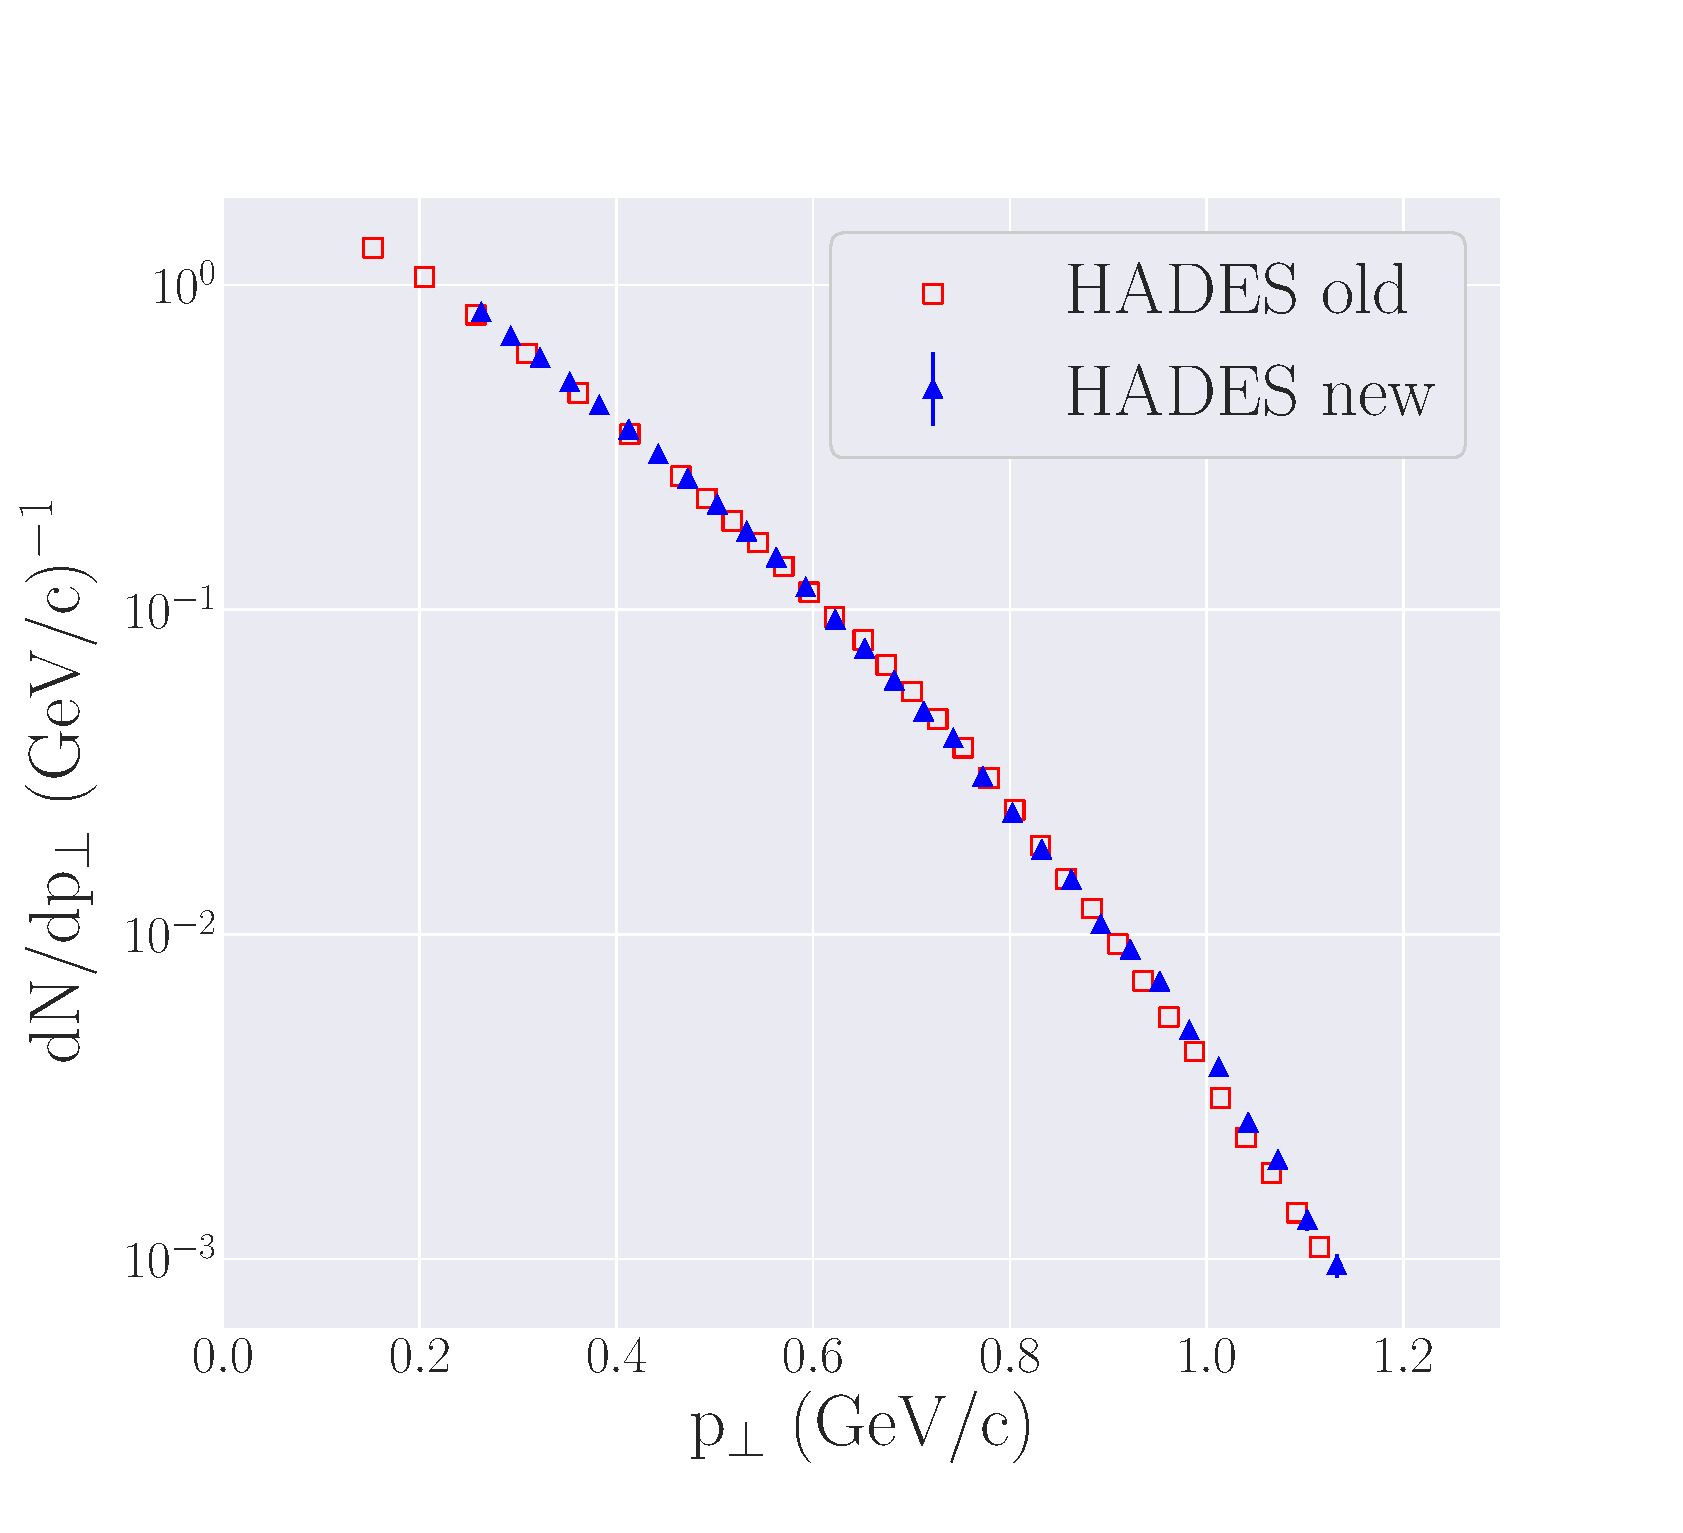
\includegraphics[width=0.95\textwidth] {PtPionN.eps}%
	\caption{\label{Comp_HADES_pt1} 
		The transverse momentum, $p_{T}$, distribution of $\pi^{-}$ for the selected rapidity, 
		$y_{lab}$, of 0.2 $<$ $y_{lab}$ $<$ 1.8, measured at HADES in $p+Nb$ at 3.5 GeV proton beam energy.
		Comparison of the results of current analysis (blue triangles) with the former studies of inclusive pion production performed at HADES 
		(gray rectangles) \cite{AgakishievPionP}. 
		Despite of the various analysis schemes used the results of both of them agree very well.
	}
\end{figure}

\subsection{\label{spal_data} Low energy spallation data}

The double differential cross section for light charged nuclear products were measured in a few dedicated experiments. 
Here the comparison will be done to the results obtained for proton-nucleus collision by PISA collaboration 
%\cite{FID17A} (and references therein) 
and HARP-CDP collaboration. 
%\cite{HARP_CDP_Al_2012} (and references therein). 
Data provided by PISA cover broad range of target nuclei (from C to Au) bombarded by protons of 1.2, 1.9 and 2.5 GeV energy \cite{bubak2007non,budzanowski2008competition,budzanowski2009variation,budzanowski2010comparison,fidelus2014sequential,fidelus2017non}. 
The HARP-CDP collaboration provided the proton and pion spectra for proton induced reaction on some atomic nuclei from Be to Pb 
%p+Cu and p+Ta collisions
at 4.1 GeV proton bombarding energy  \cite{HARP_CDP_Be1_2009,HARP_CDP_Be2_2009,HARP_CDP_Ta_2009,HARP_CDP_Cu_2009,HARP_CDP_C_2010,HARP_CDP_Sn_2011,HARP_CDP_Al_2012}.

In fig. \ref{Comp_PISA_HARP_pdt} the examples of production cross sections for 
$p$ (upper panel), $d$ (middle panel) and $t$ (lower panel) measured at HADES 
for $p+^{93}Nb$ @3.5 GeV and registered at laboratory emission angle $\theta$ = 65$^{\circ}$ are presented. 
The HADES results for protons are compared to the results of PISA measured for reaction 
of $p+^{nat.}Ag$ @2.5 GeV \cite{fidelus2017non} and the results of HARP-CDP 
registered for $p+^{64}Cu$ reaction at 4.1 GeV impinging proton energy \cite{HARP_CDP_Cu_2009}. 
Taking into account the target mass dependence of the cross sections 
and the similar beams energies the results are in very good agreement. 
HADES deuteron and triton production cross sections are compared to the results of PISA 
collected for the $p+^{nat.}Ag$ @2.5 GeV reaction \cite{fidelus2017non}. 
Excellent agreement about HADES and PISA results is observed. 
The agreement of the magnitudes and the slopes of PISA, HARP-CDP and HADES distributions 
for all registered H isotopes proves the correctness of the 
data selection and analysis used in this work. 


\begin{figure}
	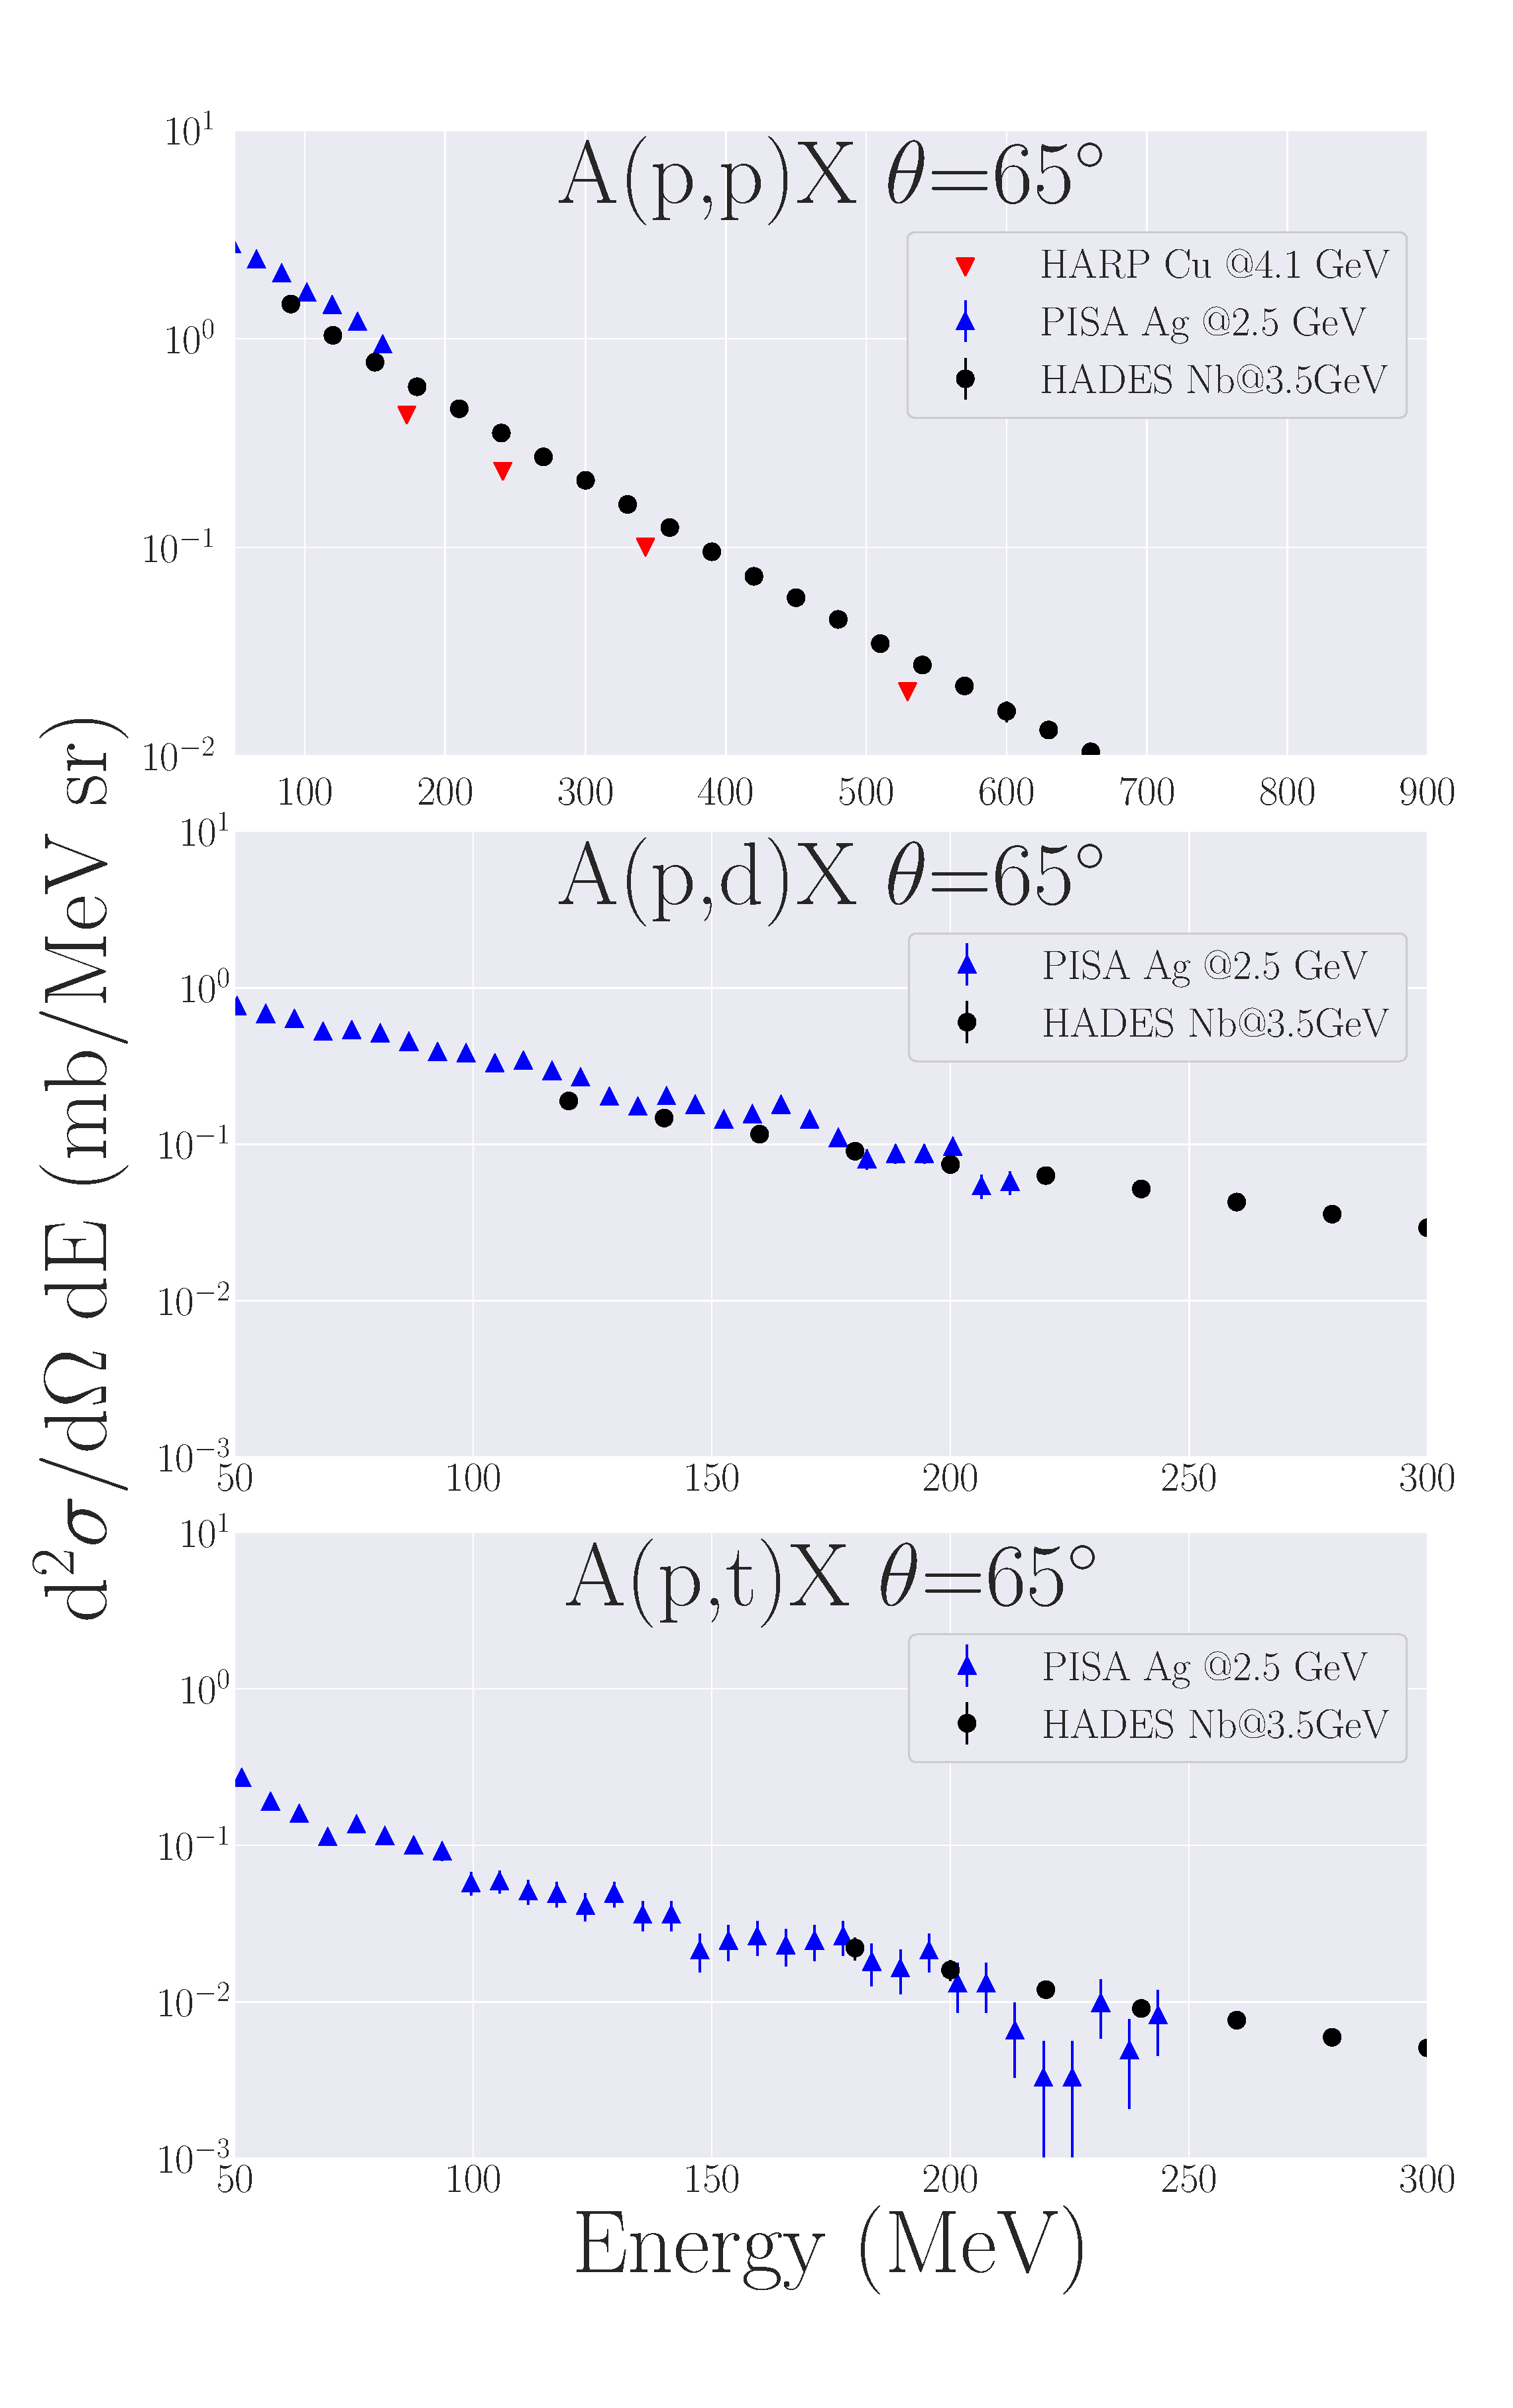
\includegraphics[width=0.4\textwidth]{all_harp_pisa.eps}
	\caption{\label{Comp_PISA_HARP_pdt} 
		Examples of double differential cross sections for $p$ (upper panel), $d$ (middle panel) and $t$ 
		(lower panel) measured at HADES 
		at $\theta$ = 65$^{\circ}$ laboratory emission angle in reaction $p+^{93}Nb$ at 
		3.5 GeV beam energy.  They are confronted with the former results of spallation  
		experiment PISA \cite{fidelus2017non} for the same isotopes and detection angle. 
		The PISA data were measured with the use of $^{nat}Ag$ target and 
		for proton beam energy of 2.5 GeV. The comparison proves the good agreement of the magnitudes 
		and shapes of the distributions of both experiments. The double differential production 
		cross sections for $p$ are compared also to the results obtained in HARP-CDP experiment 
		for the same detection angle but for reaction of  
		$p+^{65}Cu$ at 4.1 GeV \cite{HARP_CDP_Cu_2009}. The small differences in the magnitudes 
		of $p$ distributions  resulting from various experiments are due to expected 
		target mass and proton beam energy dependence of the production cross section. 
	}
\end{figure}
\subsection{\label{pion_data} Mid-energy pion spectra}

For the verification of the correctness of HADES results for $\pi^{+}$ production 
cross section the comparison to the results of 
HARP-CDP experiment was performed. This comparison is shown in fig. \ref{Comp_HARP_pip}. 
The HARP-CDP data were collected for reaction where the proton beam of energy 4.1 GeV 
bombarded the $^{64}Cu$ \cite{HARP_CDP_Cu_2009} and $^{181}Ta$ \cite{HARP_CDP_Ta_2009} targets. 
The shapes of energy distributions of $\pi^{+}$ measured at two angles (65$^{\circ}$ and 80$^{\circ}$) 
are practically the same for all tree targets.
Since the proton beam energies in both experiments were similar the observed differences 
in the magnitudes of cross sections are practically only due to target masses and 
follow expected sequence of increase of the production cross section with increase 
of the target mass number A. This fact permits the conclusion that 
the double differential cross sections for production of $\pi^{+}$ measured at HADES agree 
well with the similar results obtained by HARP-CDP collaboration.


\begin{figure}[!h]
	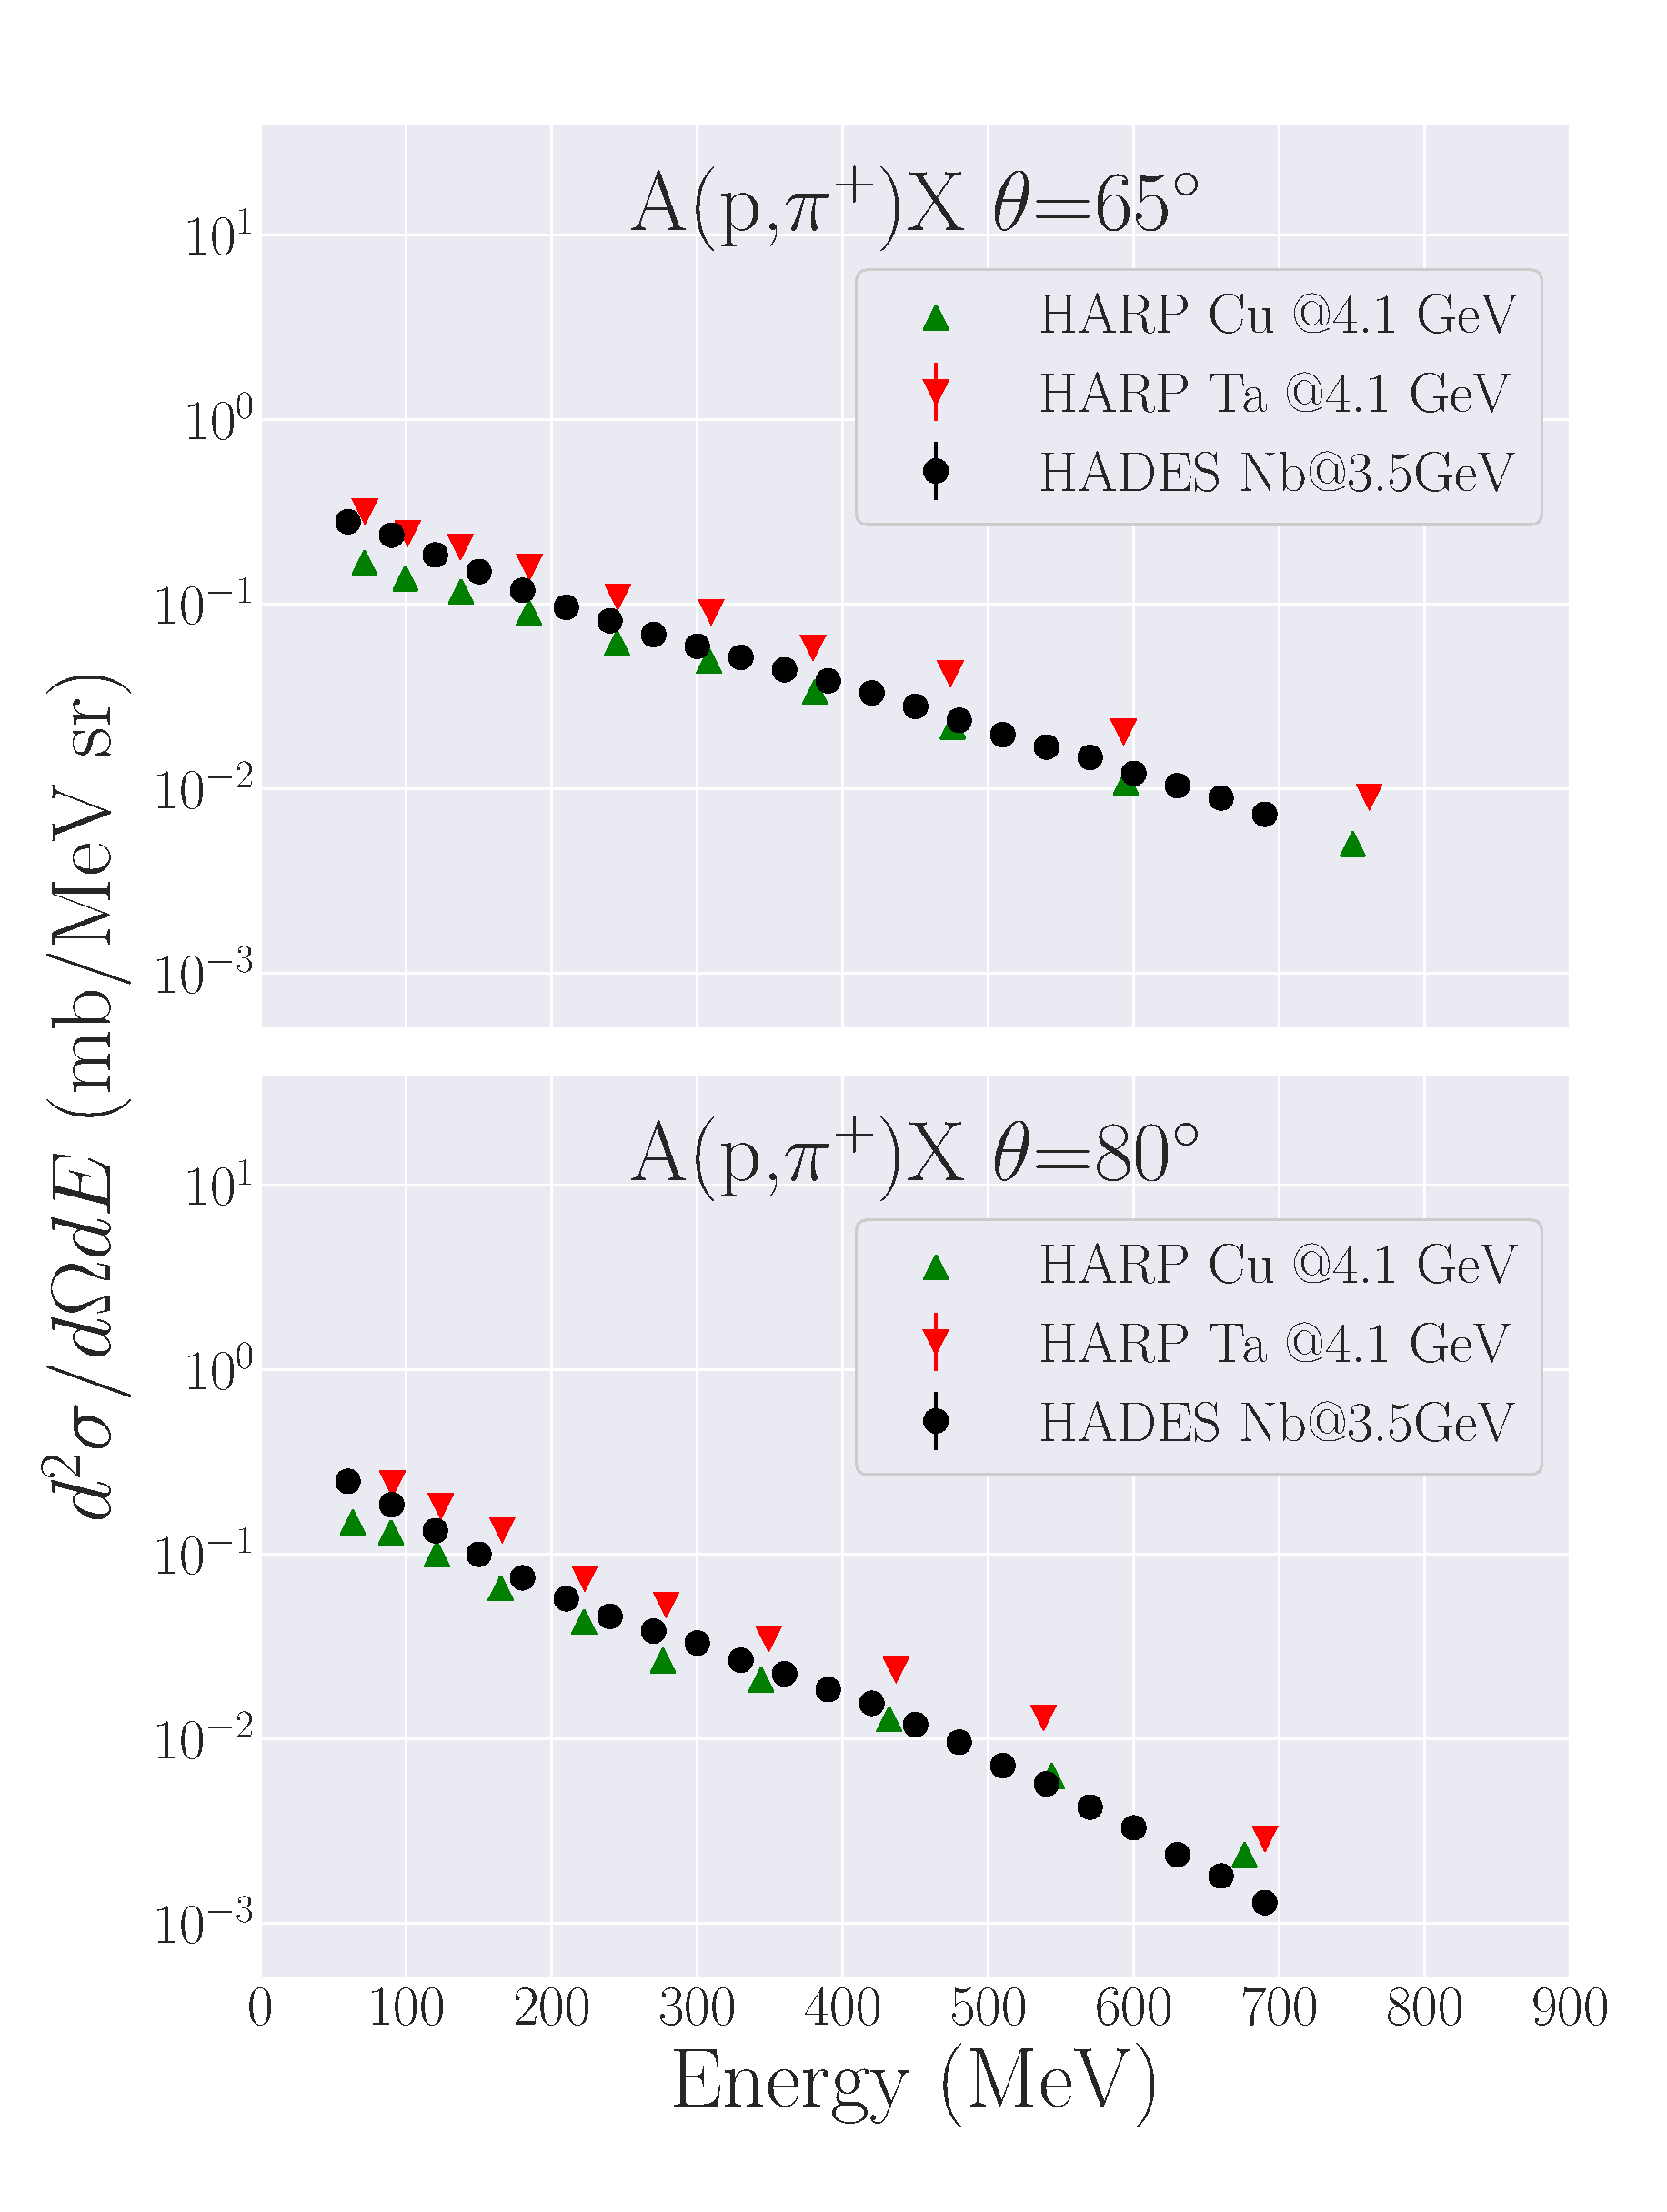
\includegraphics[width=0.75\textwidth] {PionPositive_harp_pisa.eps}%
	\caption{\label{Comp_HARP_pip} 
		Examples of double differential cross sections measured at two emission angles 
		($\theta$ = 65$^{\circ}$ - left panel, and $\theta$ = 80$^{\circ}$ - right panel) 
		at HADES for $\pi^{+}$ for $p+^{93}Nb$ @3.5 GeV (black dots). 
		They are compared to the similar results of HARP-CDP collaboration but measured for 4.1 GeV proton 
		beam impinging on $^{64}Cu$ (green triangles) \cite{HARP_CDP_Cu_2009} and $^{181}Ta$ 
		(red triangles) \cite{HARP_CDP_Ta_2009} targets.
		Taking into account the expected cross section differences due to various target masses 
		the good agreement of distributions obtained in both experiments is confirmed.
	}
\end{figure}

\ \\

Since the detection conditions during the $p+^{93}Nb$ run at 3.5 GeV beam energy were 
not optimized for registration of the single spectra of $p$,  $d$,  $t$, $\pi^{+}$ 
and $\pi^{-}$, the effort were undertaken to test if the applied analysis scheme 
including the particle identification, the background reduction and subtraction, 
the efficiency and acceptance corrections, the absolute normalization and the error 
estimation are sufficiently powerful and reliable. 
Very good agreement of the present data with those obtained in the experiments, 
which used completely different methods of measurements 
proves reliability of the present data processing.
----- kp ----------\\

In the course of the examinations of the mechanisms acting during nuclear spallation and the developments of more and more accurate theoretical models describing these phenomena it become clear that the usefulness of the observables provided by experiments increases with their exclusiveness.
The simple observable like particle multiplicities or the total production cross section are less sensitive for details of interplaying mechanisms than e.g. the angular or energy distributions of the reaction products or their coincidences.
Of course, the most demanded would be the experiment allowing for complete registration of all reaction products in 4$\pi$ geometry and in the whole kinematic range. Unfortunately such experiments are not planned. Thus, taking advantage of the broad acceptance of HADES apparatus and 
of its magnetic spectrometer it was decided that the double differential cross sections ($d^2\sigma/d\Omega dE$) will be derived as a first portion of spallation data delivered by HADES. 

In the view of the actual conditions under which the data were collected (trigger requiring coincidence of at least 3 particles, T-o-F reconstructed from coincidence with a fast particle) perhaps the more straightforward 
would be to derive the coincidence cross section ($d^4\sigma/d\Omega_1 d\Omega_2 dE1 dE2$) at the beginning. But in order to verify the quality of the analysis method applied for particle identification and normalisation 
of the distributions it was decide to provide first the double differential cross section for single particle. It is motivated by the existence in the literature of the experimental results of the same type which can serve as a benchmark for the analysis method presented in this thesis. The verification of the method 
with more exclusive distributions would be not possible, since such data do not exists.

As it will be shown later, the verification of the method is very promising it motivates the HADES group to the perform the analysis of more exclusive observables in the next step the analysis of the spallation data.

The double differential cross section are already good and sensitive observable useful for the model developers. But for the more general use of  the current HADES results the examples of them will be shown also in other representations - as the distributions of transverse momenta or as transverse masses distributions. 

In order to create the ($d^2\sigma/d\Omega dE$) 
%and the (d2σ/dΩ1dΩ2 ) 
cross sections for the $\pi$ and $H$ isotopes from p+Nb reaction at 3.5 GeV bombarding energy 
the following steps of data selection had to be done:
\begin{itemize}
\item Definition of the rough selection cuts (1-st level) for proton, deuteron, triton and pions with the use of the 
mass-momentum distribution;
\item For such preselected data creation of $dE/dx_{(MDC)}  vs. momentum$ plots;
\item The projection of $dE/dx_{(MDC)}$ distributions in momentum slices of
25 MeV$/$c to the $dE/dx$ axis. The asymmetric Gaussian fit to each particular distribution in order to define the identification cuts. 
The cuts (2-nd level) are fixed by selection of given 
sigmas of the fitted functions;
\item For data selected as above creation of $dE/dx_{(TOF)}$ and 
$dE/dx_{(TOFino)} vs. momentum$ distributions.
\item The projections of these distributions to the $dE/dx$ axes and the 
fits of the asymmetric Gaussian functions  
to the $dE/dx$ distributions for each of 25 MeV$/$c momentum bin. 
In this way the definition of the 3-rd level of identification cuts at selected sigma of the fitted distributions.
\item Created 3-rd level cuts are used to identify the relevant species for the data where cuts of level 1 a and level 2 were disregarded.
\end{itemize}


 
%----- kp ----------\\

 



In order to create the ($d^2\sigma/d\Omega dE$) and the ($d^2\sigma/d\Omega_1 d\Omega_2$) cross sections the data collected in p+Nb reaction at 3.5 GeV bombarding energy will be used.  The detection system of the HADES experiment is shown in Fig. 3. 
The toroidal magnetic field of HADES system for the momentum measurement together with the precise tracking of 4 layer Mini Drift Chambers (MDC) and particle identification (PID) based on dE/dx information from MDC, TOF and TOFino scintillators will allow to create the double-differential cross sections distributions ($d^2\sigma/d\Omega dE$) for LPCs and for pions for emission angles between 18O and 85O. The energy range will cover their almost whole kinematic range. It means that the energy distributions of protons will range from about 50 MeV until about 2.6 GeV (cf. Fig. 2 and 3). It has to be stressed here again that in dedicated experiments oriented for spallation physics [4-9] the particle detection and identification were possible only for energies lower than ~200 MeV cf. Fig. 1 and [3].  
\begin{figure}
	% Requires \usepackage{graphicx}
	\centering
	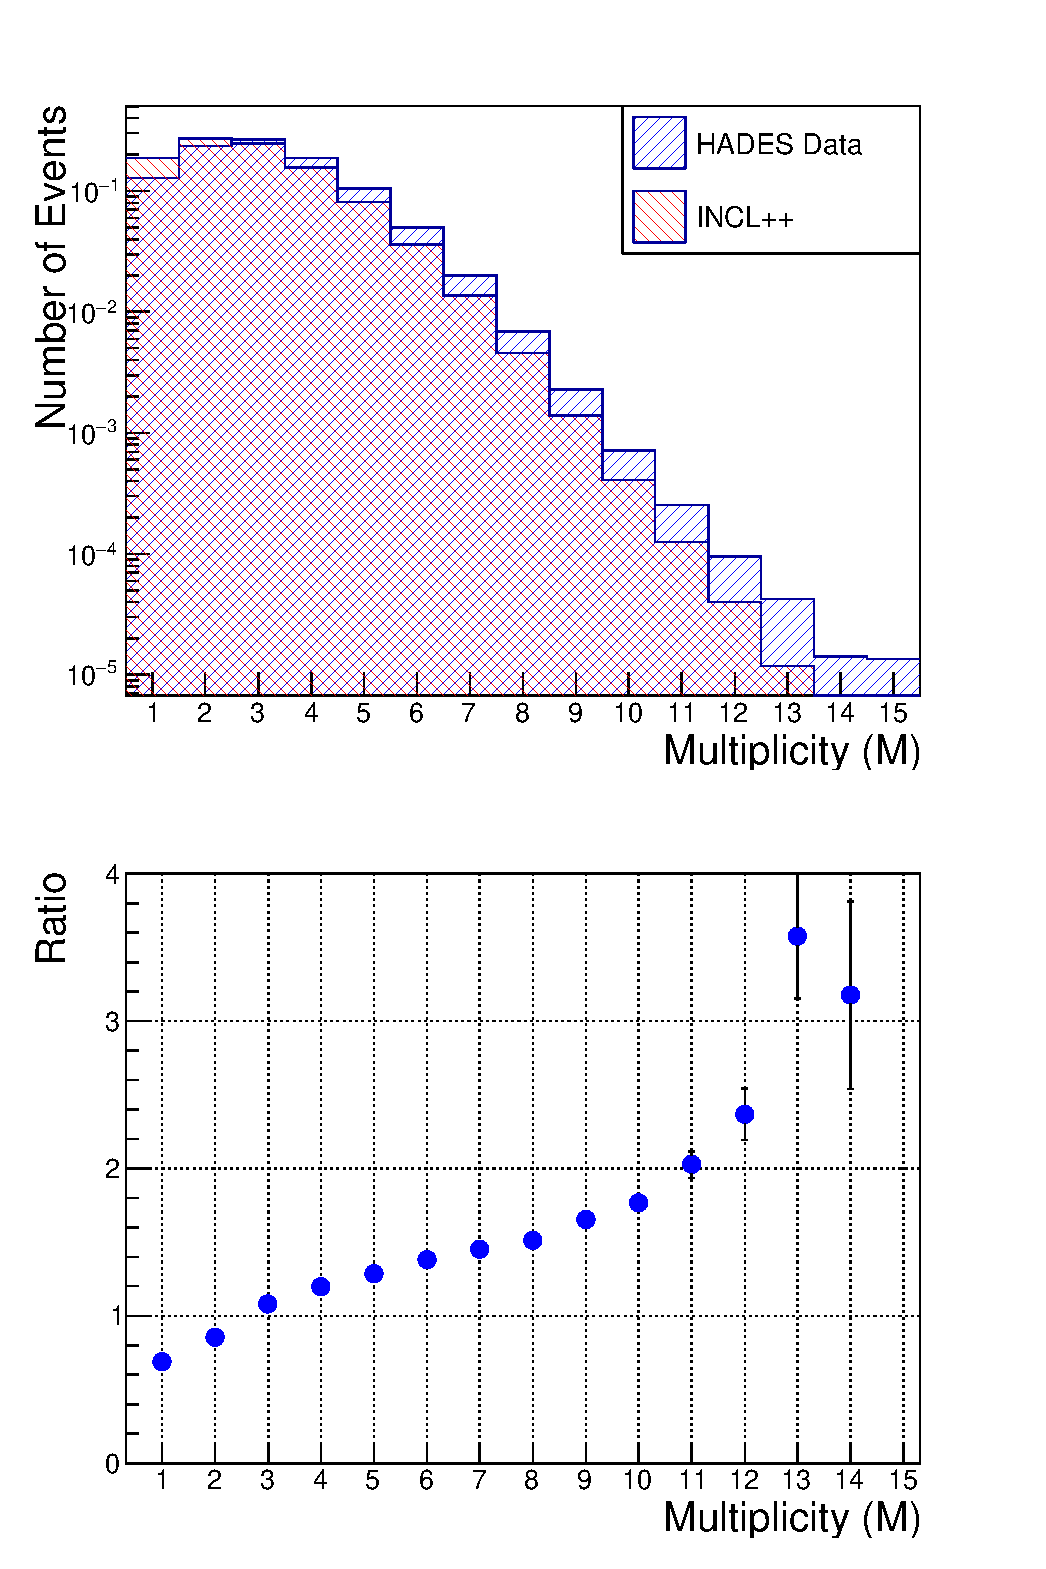
\includegraphics[width=120mm]{MultINCL.eps}
	\caption{\label{Eff_simulations} The comparison of simulated and detected multiplicities (M) of charged particles in the HADES 
detection system for the $p+Nb$ run at 3.5 GeV. Simulations were performed with the use of the standard HADES tools 
(HGeant+Hydra \cite{}) where as an event generator the INCL++ model has been utilized. The decent agreement of both 
distribution for M $\ge$ 3 permitted to use this combination of tools for efficiency corrections for the measured reaction 
products. Please, note that the disagreement of simulated and registered multiplicities for M $<$ 3 is an effect of 
trigger condition demanding charged particles multiplicity of M $\ge$ 3. 
}
\end{figure}
% \begin{figure}
% 	% Requires \usepackage{graphicx}
% 	\centering\
% 	\includegraphics{cuts}
% 	\caption{The scatter plot of dE/dx (MDC) vs. momentum for protons. The cut obtained from 
% 		the asymmetric Gaussian fits is shown. The theoretical calculation of energy loss according to Bethe-Bloch formula is shown as well with the red line.}
% 	\label{MDCcut}
% \end{figure}
Pion and Light Charged Particle identification in HADES experiment 

For PID in HADES experiment the information from Time of Flight, the dE/dx in MDC detector and dE/dx in TOF and TOFino detectors are used. However, in a few data sets the information on Time of Flight is not available due to hardware constraints. But even in this case, the time of flight can be reconstructed with the use of information from TOF and TOFino detectors (which are the STOP detectors for the time of Flight measurement) and reconstructed track of fast particles like $\pi-$.  Such a reference particle has to be detected together with other reaction products what impose the specific the trigger condition, unfavorable measurement of the absolute cross section for single particles. Thus, for creation of a double differential cross section of LCP and pions, the PID of these particles is restricted only to information gained from dE/dx measurements. Nevertheless, the reconstructed Time of Flight of reaction products can be used for rough particle selection with the mass vs. momentum cuts as it is shown in Fig. 5.
In order to obtain the single spectra of LCP and pions the combination of identification methods is done in the following way:
\begin{figure}
	% Requires \usepackage{graphicx}
	\centering\
	\includegraphics[width=120mm]{cuts2}
	\caption{The scatter plot of dE/dx(TOFino) vs. momentum (upper panel) and dE/dx(TOF) vs. momentum (lower panel) for proton showing the cuts selecting the protons.}
	\label{TofCut}
\end{figure}
1. The mass-momentum distribution is used to define the rough selection cuts for proton, deuteron, triton and pions (cf. Fig. 5).



Fig. 5. The scatter plot of momentum vs. mass for mesons and LPC registered and identified with the HADES detection system.


2. For the selected particles the dE/dx (MDC) vs. momentum plots are done (cf. Example in fig. 6).

3. The projection of dE/dx (MDC) distributions in momentum slices of 25 MeV/c is done. The asymmetric Gaussian fit is applied to each particular distribution in order to define the cuts. The cuts are fixed at (mean 1.5 sigmas) of the fitted functions.

4. Using both the MDC dE/dx (MDC) cut and mass cuts the dE/dx (TOF) and dE/dx (TOFino) vs. momentum are done. The procedure of fitting of the asymmetric Gaussian distribution to the 25 MeV/c momentum slices is applied again.

5. After the final cuts are defined, they are applied to the data set where the mass cut is not used.


\subsection{issues in data analysis}
\subsection{Description of analysis}
\subsection{Establishing of systematic uncertainties}
